%%%%%%%%%%%%%%%%%%%%%%%%%%%%%%%%%
%Preamble
%%%%%%%%%%%%%%%%%%%%%%%%%%%%%%%%%

\PassOptionsToPackage{usenames, dvipsnames}{xcolor}

\documentclass[a4paper, table]{article}
\usepackage[english]{babel}
\usepackage[margin=1in]{geometry}
\usepackage[ruled, vlined]{algorithm2e}

\usepackage{amsfonts}
\usepackage{setspace,graphicx,epstopdf,amsmath}
\usepackage{marginnote, datetime, url, enumitem, subfigure}

%Journal Style
%JFE looks nice, JF looks awful
	\usepackage{amsthm}
	\usepackage{jfe}

%Bibliography Stuff
	%Use natbib even though it's old because it's compliant with journal styles
	%Actual bibliography style etc are specified where you actually want it
	\usepackage{natbib}

%Fluff
	\linespread{1.3}

%Neural Network Packages
	\usepackage{neuralnetwork}
	\usepackage{xpatch}
	\makeatletter
	% \linklayers have \nn@lastnode instead of \lastnode,
	% patch it to replace the former with the latter, and similar for thisnode
	\xpatchcmd{\linklayers}{\nn@lastnode}{\lastnode}{}{}
	\xpatchcmd{\linklayers}{\nn@thisnode}{\thisnode}{}{}
	\makeatother
	
%Regression Tree
	\usepackage{tikz,forest}
	\usetikzlibrary{arrows.meta}
	
	\forestset{
		.style={
			for tree={
				base=bottom,
				child anchor=north,
				align=center,
				s sep+=1cm,
				straight edge/.style={
					edge path={\noexpand\path[\forestoption{edge},thick,-{Latex}] 
						(!u.parent anchor) -- (.child anchor);}
				},
				if n children={0}
				{tier=word, draw, thick, rectangle}
				{draw, diamond, thick, aspect=2},
				if n=1{%
					edge path={\noexpand\path[\forestoption{edge},thick,-{Latex}] 
						(!u.parent anchor) -| (.child anchor) node[pos=.2, above] {Y};}
				}{
					edge path={\noexpand\path[\forestoption{edge},thick,-{Latex}] 
						(!u.parent anchor) -| (.child anchor) node[pos=.2, above] {N};}
				}
			}
		}
	}

\usepackage{lscape}
\usepackage{longtable}

%%TODONOTE commands
\usepackage[colorinlistoftodos]{todonotes}
\newcommand{\smalltodo}[2][] {\todo[caption={#2}, size=\scriptsize,%
	fancyline,#1]{\begin{spacing}{.5}#2\end{spacing}}}
\newcommand{\rhs}[2][]{\smalltodo[color=green!30,#1]{{\bf RS:} #2}}
%%

%Graphs
\usepackage{tikz}
\usepackage{pgfplots}
\graphicspath{{../Results/}}

%Coloured Tables

%%%%%%%%%%%%%%%%%%%%%%%%%%%%%%
%%Title and other fluff, just before document start
%%%%%%%%%%%%%%%%%%%%%%%%%%%%%%

%Hyperref apparently is a big package and causes a lot of issues, so it's recommended to load this last

\usepackage{hyperref}

%Gets rid of the neon green boxes around boxes

\usepackage[]{xcolor}

\hypersetup{
	colorlinks,
	linkcolor = {red!50!black},
	citecolor = {blue!50!black},
	urlcolor = {blue!80!black}
}

\title{Evaluation of Machine Learning in Empirical Asset Pricing}
\author{Ze Yu Zhong}

%%%%%%%%%%%%%%%%%%%%%%%%%%%%%%%
%%BEGIN DOCUMENT
%%%%%%%%%%%%%%%%%%%%%%%%%%%%%%%

\begin{document}

\maketitle

\tableofcontents

%%%%%%%%%%%%%%%%%%%%%%%%%%%%%%%%%%%%%%%%%%%%%%%%%%%%%%%%%%%%%%%%%%%%%%%%%%%%%%%%%%%%%%%%%%%%%%%%%%%%%

\section{Introduction}

\subsection{Topic}

This thesis aims to evaluate the application of machine learning algorithms in empirical asset pricing. While there has been significant recent interest in applying machine learning to the problem of predicting asset returns, there is little literature that focuses on how well these algorithms are at capturing true underlying variables in determining stock returns. 12 different simulated datasets ranging from linear to highly non-linear data generating processes incorporating observed phenomena of cross sectional correlation, persistence, and stochastic volatility, in addition to real world data will be used to assess the performance of linear models, elastic net models, random forests and neural networks. Model performance will be assessed according to their out of sample Mean Absolute Error, Root Mean Square Error, and Predictive $R^2$, in addition to whether or not they were able to identify the correct variables in the data generating process according to a variable importance metric.

\subsection{Background Literature and Motivations}

This paper is motivated by evaluating the performance of machine learning algorithms in empirical asset pricing, focusing on how well they deal with the many unique problems in financial returns data. Here, we define ``performance" to refer to two forms of metrics conventional in the literature: $R^2$ (and more specifically, out of sample $R^2$), and forecast errors (see \ref{model_evaluation} for more details).

We first begin by defining ``factors" with the more contemporary definition as suggested by \cite{harvey__2016}: a collection of regressors to be used in pricing returns that can be used to proxy for unknown underlying risk factors due to their correlation with cross sectional returns. Most notably, their definition rejects the more strict view that risk factors should be variables that have unpredictable variation through time, and that they should be able explain cross sectional return patterns. \cite{harvey__2016} further groups factors into the two broad categories of ``common" and individual firm ``characteristics." ``Common" factors under this definition can be viewed as proxies for sources of risk constant across all firms, such as macroeconomic variables. They note that individual firm characteristics are unlikely to satisfy the more strict definition because they are often pre-known and display limited time series variation.

Because of this less strict definition, factors introduced and used in the literature often exhibit properties which makes them unsuitable for inclusion in models, such as high persistence, high levels of non-stationarity and cross sectional correlation. 

\cite{goetzmann_testing_1993} and \cite{ang_stock_2006} note the persistence present in dividend ratio factors. This means that movements in dividend ratios are dominated by movements in price and therefore dividend ratios are correlated with lagged dependent variables on the right hand side of the regression equation. This violates the assumptions of exogeneous regressors (independent from the error term) required for traditional regression models (ordinary least squares) to be unbiased, resulting in t statistics which are biased upwards and increase with time horizon due to autocorrelated errors. Importantly, \cite{goetzmann_testing_1993} show that corrections to t statistics using the Generalized Method of Moments and Newey-West standard errors also appear to be biased upwards, making them unreliable. 

\cite{goyal_predicting_2003} provide a more comprehensive study on the performance of lagged dividend price ratios, with specific focus on out of sample predictive performance both in terms of $R^2$ and forecast errors. They conclude that while models incorporating dividend related factors were able to achieve higher in sample performance prior to 1990 than the historical mean, they could not have outperformed the historical mean \textit{out of sample}. \cite{goyal_predicting_2003} attribute this to the increasing persistence and non-stationarity of dividend ratios, noting that they have become like random walks as of 2001. This mirrors the sentiment of (\cite{lettau_consumption_2001}, \cite{schwert_anomalies_2003} and others) who conclude that models incorporating dividend ratios seemed to break down in the 2000s due to a changing economic environment despite having performed well in the 1990s.

Despite the controversy, the prevailing tone within the literature was that various factors such as dividend ratios, earnings price ratio, interest and inflation and other financial indicators were able to predict excess returns, with \cite{lettau_consumption_2001} remarking that this was now ``widely accepted." However, \cite{welch_comprehensive_2008} extend upon the work of \cite{goyal_predicting_2003} by including a more comprehensive set of variables and time horizons. They conclude that not a single variable had any statistical forecasting power. Crucially, they demonstrate the non-robustness of models incorporating these factors by showing that the significance values of some factors change with the choice of sample periods.

Despite this, the literature has continued to produce more factors: quantitative trading firms were using 81 factor models as the norm by 2014 \citep{hsu_finding_2014}, and \cite{harvey_census_2019} currently document well over 600 different factors suggested in the literature. 

The dramatic increase in the number of factors alone poses challenges to traditional statistical techniques. \cite{harvey__2016} detail the false discovery problem when the number of potential factors is extremely high. The significance of a factor in a traditional regression setting is determined by a single hypothesis test, which by construction carries a level of significance $\alpha$ controlling the type I error rate: the probability of rejecting a "null" hypothesis that a factor is not important, and hence incorrectly concluding that it is significant. When the number of potential factors is large, it is very likely that a factor will be concluded as significant by pure chance. For example, a factor model consisting of 600 factors would find around 30 factors significant by chance at the 5\% significance level. \cite{harvey__2016} produce a multiple testing framework to mitigate this, and conclude that many of the historically discovered would have been deemed significant by chance.

Furthermore, \cite{feng_taming_2019} note that the number of potential factors discovered in the literature has increased to the same scale as, if not greater, than the number of stocks considered in a typical portfolio, or the time horizon, producing highly inefficient covariances in a standard cross sectional regression. Moreover, when the number of factors exceeds the sample size, traditional cross sectional regressions become infeasible and do not produce solutions altogether. 

It does not help that many factors are cross sectionally correlated, meaning that factors which are discovered to be significant may simply be so because they are correlated with a true, underlying factor and do not provide independent information themselves, a concern which \cite{cochrane_presidential_2011} calls the multidimensional challenge. \cite{freyberger_dissecting_2017} notes that this is especially challenging for traditional regression models, which make strong functional form assumptions and are sensitive to outliers. 

\rhs{More reasoning on why ML is good here}

More recently, machine learning algorithms have emerged within the literature and appear to be well suited to the task of predicting asset returns. The definition of machine learning can be vague and is often context specific; \cite{hastie_elements_2009} in \textit{An Introduction to Statistical Learning} describes statistical (machine) learning as a vast set of tools for understanding data, and \textit{supervised} learning specifically as the process of building a statistical model for the prediction or estimation of an output based on input(s). In the context of asset pricing, we use the term to refer to a diverse collection of:

\begin{enumerate}
	\item high-dimensional models for statistical prediction, 
	\item the ``regularization" methods for model selection and mitigation of over-fitting input data, 
	\item and the efficient systematic methods for searching potential model specifications.
\end{enumerate}

\rhs{provide some examples of regularization, such as train vs validation}

The high dimensional and hence flexible nature of machine learning brings more hope to approximating unknown and likely complex data generating processes that underlie excess returns. The flexibility however, comes at a cost of potentially over-fitting in sample data (referred to as training data in the machine learning literature), generalizing poorly and producing poor forecasts. The regularization aspect of machine learning explicitly guards against over-fitting problems and emphasizes out of sample performance. The most explicit example of regularization is the splitting of the dataset into an explicit "training" set used for model fitting, and a "test" set withheld and used solely for evaluating out of sample performance. Finally, machine learning offers tools which are designed to produce an optimal model specification from all possible models with manageable computational cost, all in a systematically consistent way.

\rhs{better linkage needed here}

\cite{kozak_shrinking_2017}, \cite{rapach_forecasting_2013} and \cite{freyberger_dissecting_2017} all apply shrinkage and selection methods from machine learning in factor selection.  

Most importantly, portfolios constructed using machine learning have been demonstrated to outperform traditional models in predicting stock returns (\cite{gu_empirical_2018}, \cite{hsu_finding_2014} and \cite{feng_deep_2018}) in terms of out of sample predictive $R^2$ and Sharpe Ratios. \cite{gu_empirical_2018} attribute this to machine learning's ability to evaluate and consider non-linear complexities among factors that cannot be feasibly achieved using traditional techniques. 

\rhs{emphasize why the limited simulation design is a problem}

However, there is little work done on how machine learning actually recognises and deals with the challenges of returns prediction documented in the literature. Prior work has been done by \cite{gu_empirical_2018}, however; only basic simulation designs which were not representative of real financial data were considered. This is problematic, 

Furthermore, \cite{feng_deep_2018} in particular use cross validation as part of their model building procedure, destroying the temporal aspect of returns data, in addition to only using a handful of factors. \cite{gu_empirical_2018} produce models using a training sample which ends in the 1970s to ultimately produce forecasts for the most recent 30 years. Given the non-robustness of financial data affecting even traditional regressions which are considered to be more inflexible, more research should be done into the robustness of more flexible machine learning methods with regards to sample selection and periods of returns predictability.

For the aspect of factor selection specifically, \cite{gu_empirical_2018} concludes that all of the machine methods agree on the same subset of important factors. However, while their factor importance metrics for regression-tree based methods and neural networks (the most complex methods considered) are mostly consistent, they have differences in terms of the relative importance of each factor, in addition to completely different conclusions for the dividend yield factor.

This paper will be the first in focusing on how machine learning algorithms perform in environments with problems exhibited by financial returns data through extending the simulation designs of \cite{gu_empirical_2018}. In addition, these algorithms will once again be evaluated on real world data, but with only more recent and representative data included in order to test their short term robustness in predicting stock returns. These two aspects of the study together are able to offer a better glimpse as to how ``black box" machine learning algorithms deal with the challenges present in asset pricing, if at all.

%\subsection{Main Findings}

%\rhs{Pending}

%\subsection{Limitations of Machine Learning}

%Machine learning excels at prediction problems, namely estimating \( E(r_{i, t+1}|\mathcal{F}_t) \), where \( r_{i, t+1} \) is an asset's excess return over the risk free rate, and \( \mathcal{F}_t \) is the set of all information (including unobservable) available to market participants in this context.

%This means that machine learning algorithms do not, nor do they aim to, explain how the market works in terms of underlying dynamics and equilibria. Though a machine learning algorithm may be able to identify patterns that otherwise cannot be easily found, an economist is still required to analyse these patterns to construct and hypothesize economic theory.

%%%%%%%%%%%%%%%%%%%%%%%%%%%%%%%%%%%%%%%%%%%%%%%%%%%%%%%%%%%%%%%%%%%%%%%%%%%%%%%%%%%%%%%%%%%%%%%%%%%%%%%%%%%%

\section{Methodology}

\subsection{Overall Model Design}

Each model will be presented and explained so that a reader without any machine learning background can understand the basic idea behind each model. All asset excess monthly returns denoted as $r_{i, t+1}$ are modelled as an additive prediction error model conditional on the true and unobservable information set available to market participants up to and including time $t$, $\mathcal{F}_t)$:

\begin{equation}
	r_{i, t+1} = E(r_{i, t+1} | \mathcal{F}_t) + \epsilon_{i, t+1}
\end{equation}

where 

\begin{equation}
	E(r_{i, t+1} | \mathcal{F}_t) = g^*(z_{i,t})
\end{equation}

with stocks indexed as $i = 1, \dots, N$ and time domain by $t = 1, \dots, T$. $g^*(z_{i,t})$ represents the model approximation using the $P$ dimensional predictor set $z_{i,t}$. We allow $g^*(z_{i,t})$ to be a flexible function of the predictor set $z_{i,t}$, and most notably, not depend on $i$ or $t$ directly. This means that we do not re-estimate a model for each time period, or independently estimate a model for each stock. Note that $g^*(z_{i,t})$ only contains information in time $t$ for individual stock $i$, meaning that while the model and its parameters will be estimated using $\mathcal{F}_t$ for stock $i$, predictions for $r_{i, t+1}$ will only use information at time $t$ as an input, analogous to using variables lagged by one period. 

\subsection{Sample Splitting}
\label{sample_split}

\rhs{unclear, re-do slightly}

Imperative to any machine learning technique is the establishment of how the dataset is to be split into training, validation and test sets. The training set is used to initially build the model and provide initial estimates of parameters, whereas the validation set is used to tune model parameters to optimise out of sample performance, thus preventing overfitting. The validation set acts as a simulation of out of sample testing, whereas the test set is used only for evaluation, and is thus truly out of sample.

There are three main approaches to splitting temporal data (such as financial data). 

The first is to decide arbitrarily on a single training, validation and test set. This method is straightforward and the least computationally intensive, but is limited and inflexible in evaluating how models perform when more recent data is provided for training. 

The second method is a "rolling window" method, where a fixed size or "window" for the training and validation set is first chosen. This window then incrementally move forwards in time to include more recent data, with a set of forecasts for the test sets made for all possible windows.

The third is a "recursive" method, which is the same as the rolling window method, but different in that the training set always contains previous data, with only the validation set staying fixed in size and "rolling" forwards. Hence, it is also referred to as a "growing window."

Both the rolling window and recursive schemes are very computationally intensive. Therefore, a hybrid of the rolling and recursive schemes was considered: the training set is increased by one year with each refit, the validation set remains one year in length but moves forward by one year, and forecasts are made using that model for the subsequent year. The ``traditional" cross validation method of randomly sampling to determine a train and validation set was not done to maintain the temporal ordering of the data.

\subsection{Loss Function}

The choice of the loss function used in models is imperative to machine learning. The loss functions considered are Mean Absolute Error (MAE), Mean Squared Error and Root Mean Squared Error (MSE, and RMSE).

\subsubsection{Mean Absolute Error}

The mean absolute error (MAE) is simply the average magnitude of errors. Because of this, it places equal weighting to all magnitudes of errors and is more robust to outliers. 

\begin{equation}
	\text{MAE} = \frac{1}{n} \sum_{j = i}^{n} |y_j - \hat{y_j}|
\end{equation}

It should be noted that minimizing the MAE criterion is equivalent to minimizing 0.5 quantile loss.

\subsubsection{Mean Squared Error and Root Mean Squared Error}

The mean squared error (MSE) and root mean squared error (RMSE) are quadratic scoring methods. This means that they place higher weight on large errors. Models that minimize this metric are therefore more sensitive to outliers. 

\begin{align}
	\text{MSE} &= \frac{1}{n} \sum_{j = i}^{n} \left( y_j - \hat{y_j}\right) ^2 \\
	\text{RMSE} &= \sqrt{ \frac{1}{n} \sum_{j = i}^{n} \left( y_j - \hat{y_j}\right) ^2}
\end{align}

\subsection{Linear Model}

\rhs{explain how linear models struggle with high dimensionality}

The least complex model considered is the simple linear regression model. Linear models struggle with high-dimensionality. Nevertheless, despite being expected to perform poorly it was implemented as a ``control."

The simple linear model assumes that the underlying conditional expectation \( g^*(z_{i, t}) \) can be modelled as a linear function of the predictors and the parameter vector \( \theta \):

\begin{equation}
	g(z_{i, t};\theta) = z_{i, t}' \theta
\end{equation}

This model can capture non-linearities only if the predictor set \(z^*_{i, t}\) contains specified non-linear transformations or interaction terms. 

Note that computing this model with respect to minimizing the mean squared error yields the pooled ordinary least squares estimator (POLS), while minimizing the mean absolute error corresponds to quantile regression predicting the 0.5th quantile.

\subsection{Penalized Linear Model}

Penalized linear models have the same underlying statistical model as simple linear models, but differ in their addition of a new penalty term in the loss function:

\begin{equation}
	\mathcal{L(\theta;.)} = 
	\underset{\text{Loss Function}}{\underbrace{\mathcal{L(\theta)}}} + 
	\underset{\text{Penalty Term}}{\underbrace{\phi(\theta;.)}}
\end{equation}

Several choices exist for the choice of penalty function \( \phi(\theta;.) \). We restrict our scope to the popular "elastic net" penalty \citep{zou_regularization_2005}:

\begin{equation}
	\phi(\theta;\lambda,\rho) = 
	\lambda(1-\rho) \sum_{j = 1}^{P}|\theta_j| +
	\frac{1}{2} \lambda \rho \sum_{j = 1}^{P}\theta_j^2
\end{equation}

The elastic net has two hyperparameters: $\lambda$, which controls the overall magnitude of the loss, and $\rho$, which controls the shape of the penalization. 

The $\rho = 1$ case corresponds to ridge regression proposed by \cite{hoerl_ridge_1970}, which uses $l_2$ that shrinks all coefficients closer to 0, but not to 0. Ridge regression is therefore a shrinkage method which prevents coefficients from becoming too large and overpowering. For \(0 < \rho < 1\), the elastic net aims to produce parsimonious models through both shrinkage and selection.

The $\rho = 0$ case corresponds to the popular LASSO and uses absolute ($l_1$) parameter penalization proposed by \cite{tibshirani_regression_1996}, which geometrically allows the coefficients to be shrunk to 0. This allows it to impose sparsity, and can be thought of as a variable selection tool.

By combining the properties of LASSO and ridge regression, the elastic net aims to produce parsimonious models through both coefficient shrinkage and selection.

The hyperparameters $\lambda$ and $\rho$ are both tuned using the validation sample (see \ref{Algorithms}). 

\pagebreak

\subsection{Classification and Regression Trees}

Classification and regression trees are fully non-parametric models that can capture complex multi-way interactions. A tree "grows" in a series of iterations. With each iteration, a split ("branch") is made along one predictor such that it is the best split available at that stage with respect to minimizing the loss function. These steps are continued until each observation is its own node, or more commonly until the stopping criterion is met. The eventual model slices the predictor space into rectangular partitions, and predicts the unknown function $g^*(z_{i,t})$ with the average value of the outcome variable in each partition.

The prediction of a tree, $\mathcal{T}$, with \(K\) "leaves" (terminal nodes), and depth $L$ is

\begin{equation}
	g(z_{i,t};\theta,K,L) = \sum_{k=1}^{K}\theta_k\textbf{1}_{z_{i,t}\in C_k(L)}
\end{equation}

where $C_k(L)$ is one of the $K$ partitions in the model.

For this study, only recursive binary trees (the most common and easy to implement) are considered. Though trees were originally proposed and fit with respect to minimizing mean squared error, they can be grown with respect to a variety of loss functions, including mean absolute error, mean squared error:

\begin{equation}
	H(\theta, C) = \frac{1}{|C|} \sum_{z_{i,t} \in C} L(r_{i,t+1} - \theta)
\end{equation}

where $|C|$ denotes the number of observations in set C (partition). Given $C$, it is clear that the optimal choice for minimising the loss function when it is mean squared error is simply $\theta = \frac{1}{|C|} \sum_{z_{io,t}\in C}^{ }r_{i,t+1}$ i.e. the average of the partition, and the median of the partition when the loss function is mean absolute error.

Trees, grown to a deep enough level, are highly unbiased and flexible. The trade-off is their high variance and instability. Thus, an ensemble method called "Random Forest" was proposed by \cite{breiman_random_2001} to regularize trees by combining many different trees into a single prediction.

\subsection{Random Forests}
Random Forests are an extension of regression trees that attempt to address some of their problems. A random forest algorithm creates $B$ different bootstrap samples from the training dataset, fits an overfit (and hence low bias) regression tree to each dataset using only a random subset $m$ size from all available predictors (also known as dropout), and then averages their forecasts as the final output. The overfit trees means that the underlying trees has low bias, and the dropout procedure means that they have low correlation. Thus, averaging these low bias, uncorrelated trees results in a low bias, yet stable model. Specific details of the random forest algorithm are detailed in the appendix.

Random forests were the most computationally intensive, and for feasibility purposes an ensemble of only $B = 30$ trees with $m = 20$ at most was considered for the simulation study, and $B = 50$ trees with $m = 40$ at most was considered for the empirical study.

\pagebreak

\subsection{Neural Networks}

\subsubsection{Introduction}

Neural networks have theoretical underpinnings as ``universal approximators" for any function, (\cite{hornik_multilayer_1989}). They are arguably the most complex type of model available, able to capture several non-linear interactions through their many layers, hence its other name ``deep learning."  On the flipside, their high flexibility often means that they are among the most parameterized and least interpretable models, earning them the reputation as a black box model.

Per this analysis, we focus on traditional ``feed-forward" networks. The feed forward network consists of an ``input layer" of scaled data inputs, one or more ``hidden layers" which interact and non-linearly transform the inputs, and finally an output layer that aggregates the hidden layers and transform them a final time for the final output. 

More specifcally, a neural network consists of layers denoted by $l = 0, 1, \dots, L$, with $l = 0$ denoting the input layer and $l = L$ denoting the output layer, and $K^{(l)}$ denoting the number of neurons in each hidden layer. The input layer is defined using predictors, $x^{(0)} = (1, z_1, \dots, z_N)'$. The output of neuron $k$ in layer $l$ is then $x_k^{(l)}$. Next, define the vector of outputs for this layer as $x^{(l)} = (1, x_1^{(l)}, \dots, x_{K^(l)}^{(l)})'$.  The recursive output formula for the neural network at each neuron in layer $l > 0$ is then:

\begin{equation}
x_k^{(l)} = \alpha(x^{(l-1)'}\theta_k^{l-1}),
\end{equation}

where $\alpha()$ represents the activation function for that layer (see next section) with the final output

\begin{equation}
g(z;\theta) = x^{(L-1)'}\theta^{L-1}
\end{equation}

Note that the specification of a constant ``1" at the beginning of each layer is the same as specifying a bias term as is popular in other parametrizations. 

\rhs{move this paragraph elsewhere}

Neural networks with up to 5 hidden layers were considered, each named NNX where X represents the number of hidden layers. The number of neurons is each layer was chosen according to the geometric pyramid rule \citep{masters_practical_1993}: NN1 has 32 neurons, NN2 has 32 and 16 neurons in the first and second hidden layers respectively, NN3 has 32, 16, and 8 neurons, NN4 has 32, 16, 8, and 4 neurons, and NN5 has 32, 16, 8, 4, 2 neurons respectively. All units are fully connected; that is, each neurons receives input from all neurons the layer before it (see Figure \ref{Neural_Network}). This mimics the methodology in \cite{gu_empirical_2018}.

\begin{figure}
	\begin{center}
		\begin{neuralnetwork}
			%Options
			[nodespacing=12mm, layerspacing=20mm,
			maintitleheight=2.5em, layertitleheight=2.5em,
			height=9, toprow=false, nodesize=20pt, style={},
			title={}, titlestyle={}]
			\newcommand{\nodetextclear}[2]{}
		    %use \ifnum to get different labels, such as x_n on the last neuron
			\newcommand{\nodetextx}[2]{\ifnum #2=8 $x_n^{(0)}$ \else $x_#2^{(0)}$ \fi}
			\newcommand{\nodetexty}[2]{$y_#2$}
			%Hidden layer textcommands
				%32 neurons
				\newcommand{\nodetextxa}[2]{\ifnum #2=7 $x_{32}^{(1)}$ \else $x_#2^{(1)}$ \fi}
				%16 neurons
				\newcommand{\nodetextxb}[2]{\ifnum #2=6 $x_{16}^{(2)}$ \else $x_#2^{(2)}$ \fi}
				%8 neurons
				\newcommand{\nodetextxc}[2]{\ifnum #2=5 $x_{8}^{(3)}$ \else $x_#2^{(3)}$ \fi}
				\newcommand{\nodetextxd}[2]{$x_#2^{(4)}$}
				\newcommand{\nodetextxe}[2]{$x_#2^{(5)}$}
			%Input Layer
			\inputlayer[count=8, bias=false, exclude = {7}, title=Input Layer, text=\nodetextx]
			%Hidden Layer 1
			\hiddenlayer[count=7, bias=false, exclude = {6}, title=Hidden Layer 1, text=\nodetextxa] 
				\linklayers[not from = {7}, not to = {6}]
			%Hidden Layer 2
			\hiddenlayer[count=6, bias=false, exclude = {5}, title=Hidden Layer 2, text=\nodetextxb] 
				\linklayers[not from = {6}, not to = {5}]
			%Hidden Layer 3
			\hiddenlayer[count=5, bias=false, exclude = {4}, title=Hidden Layer 3, text=\nodetextxc] 
				\linklayers[not from = {5}, not to = {4}]
			%Hidden Layer 4
			\hiddenlayer[count=4, bias=false, title=Hidden Layer 4, text=\nodetextxd] 
				\linklayers[not from = {4}]
			%Hidden Layer 5
			\hiddenlayer[count=2, bias=false, title=Hidden Layer 5, text=\nodetextxe] \linklayers
			%Final Layer
			\outputlayer[count=1, title=Output Layer, text=\nodetexty] \linklayers
			% draw dots
			\path (L0-6) -- node{$\vdots$} (L0-8);
			\path (L1-5) -- node{$\vdots$} (L1-7);
			\path (L2-4) -- node{$\vdots$} (L2-6);
			\path (L3-3) -- node{$\vdots$} (L3-5);
		\end{neuralnetwork}
	\end{center}
\caption{Neural Network 5 (most complex considered), without biases terms drawn}
\label{Neural_Network}
\end{figure}

\subsubsection{Activation Function}

Several choices of activation functions exist in the literature, one of the most popular being the ReLU activation function (see \cite{lecun_deep_2015} and \cite{ramachandran_searching_2017}, among others):

\begin{equation}
	\operatorname{ReLU}(x) = max(0, x)
\end{equation}

owing to its high computational speed, ability to introduce sparseness into neural networks, and fewer vanishing gradient problems, as repeatedly applying ReLU tends to saturate less compared to other activation functions such as sigmoid and tanh. However, during the study it was observed that ReLU suffered tremendously from the "dying-ReLU problem," where ReLU neurons receive weight updates that fail to activate (output a 0), hence making it unable to receive further weight updates and learn. This resulted in networks which outputted the same value for the majority of, if not all inputs. To mitigate this, a variant of ReLU known as Leaky ReLU was used instead:

\begin{align}
	\operatorname{lReLU}(x) = 
	\begin{cases}
	x \quad &\text{if} \quad x > 0; \\
	0.01x \quad &\text{otherwise}
	\end{cases}
\end{align}

This activation function assigns a small non-zero gradient to each weight, hence enabling them to receive further weight updates.

\subsubsection{Computation}

\rhs{this, like all neural networks, is a mess. Re write}

The neural network's weight and bias parameters for each layer are estimated by minimizing the loss function with respect to the parameters, i.e. by calculating the partial derivative with respect to a specific weight or bias element.

The solution to this is typically found via backpropagation, an iterative alogrithm similar to Gauss-Newton steps and produces a local minimum. These steps can be visualized as a descent towards the local minimum of the loss function; it is thus also known as "gradient descent." Note that the lack of a global minimum is actually desirable, as global minimums tend to be overfit solutions to the problem, \citep{choromanska_loss_2014}. 
A common solution is to use ``stochastic gradient descent" (SGD) where instead of optimising the loss function with respect to the entire training sample, only a small, random subset of the data (batch) is used at each optimisation step. 

\rhs{Define learning rate more properly}

Due the noisiness (randomness) introduced by SGD, the path towards the local minimum is more of a quick ``zig zag" and has the potential to ``overshoot" the local minimum and not converge to a solution. This is typically controlled via a hyperparameter known as the learning rate, which controls the step size of each gradient descent iteration. Note that it is also common to apply a learning rate hyperparameter in non SGD environments as a way to control the magnitude of each step towards the solution to assist with convergence. The learning rate is to be tuned so that the solution path descends quickly enough to be computationally feasible, but slow enough so that it does not overshoot the local minimum and not converge. In this paper, the learning rate shrinkage algorithm which adaptively shrinks the learning rate of each individual weight separately as convergence occurs known as ADAM was employed (see \cite{kingma_adam:_2014}). It should be noted that ADAM still requires a baseline learning rate which acts as a upper bound on the learning rate to be supplied, and this was tuned manually.

\subsubsection{Batch Normalization}

``Batch normalization" is a technique for addressing a phenomenon known as internal covariate shift, a particularly prevalent problem in training deep, complex neural networks, \citep{ioffe_batch_2015}. Internal covariate shift occurs when the distributions of each layers' inputs change as the parameters of the previous layer change, resulting in the need for much slower learning rates and more careful initialization of parameters. More crucially, batch normalization has been observed to help normalizing the outputs of activation layers, alleviating issues related to vanishing or exploding gradients. By normalizing (de-meaning and variance standardizing) each training step (batch) input, the representative power of each neuron is restored. Additionally, significant gains in computational speed may also be achieved.

\subsection{Simulation Design}

\subsubsection{Overall Design}

Though \cite{gu_empirical_2018} explore the performance of machine learning on simulated returns series, their design used factors are uncorrelated across $i$, and, in particular, that the factors which enter the return equation are uncorrelated with the factors that do not enter the return equation. As note by \cite{harvey__2016} and many others, this is not what is observed in practice. 

Therefore, we simulate a latent factor model with a stochastic volatility process for excess returns  $r_{t+1}$, for $t=1,\dots,T$:

\begin{flalign}
r_{i, t+1} &= 
g\left(z_{i, t}\right) + \beta_{i,t+1}v_{t+1} + e_{i, t+1}; 
	\quad z_{i, t}=\left(1, x_{t}\right)^{\prime} \otimes c_{i, t}, 
		\quad \beta_{i, t}=\left(c_{i 1, t}, c_{i 2, t}, c_{i 3, t}\right) \\ 
e_{i, t+1} &= 
	\sigma_{i, t+1} \varepsilon_{i, t+1}; \\
\operatorname{log} (\sigma^2_{i,t+1}) &= 
	\omega + \gamma \operatorname{log} (\sigma^2_{t}) + \sigma_{u}u; 
	\quad u \sim N(0, 1)
\end{flalign}

Let $v_{t+1}$ be a $3\times 1$ vector of errors, and $w_{t+1} \sim N(0, 1)$ and $\varepsilon_{i,t+1} \sim N(0, 1)$ scalar error terms. The parameters of these are tuned such that the R squared for each individual return series was around 5\%, and the annualized volatility of each return series approximately 22\%, as is often observed empirically.

The matrix $C_t$ is an $N\times P_c$ vector of latent factors, where the first three columns correspond to $\beta_{i,t}$, across the $1\leq i\leq N$ dimensions, while the remaining $P_c-3$ factors do not enter the return equation. The $P_x\times1$ vector $x_t$ is a $3 \times 1$ multivariate time series, and $\varepsilon_{t+1}$ is a $N\times 1$ vector of idiosyncratic errors. 

\subsubsection{Simulating Characteristics}

A simulation mechanism for $C_t$ that gives some correlation across the factors and across time was used. First consider drawing normal random numbers for each $1\leq i\leq N$ and $1\leq j\leq P_{c}$, according to 

\begin{equation}
	\overline{c}_{i j, t} = \rho_{j} \overline{c}_{i j, t-1}+\epsilon_{i j, t} ;
	\quad \rho_{j} \sim \mathcal{U} \left( \frac{1}{2},1 \right) 
\end{equation}

Then, define the matrix 

\begin{equation}
	B:=\Lambda\Lambda' + \frac{1}{10}\mathbb{I}_{n}, \quad
	\Lambda_i = (\lambda_{i1},\dots,\lambda_{i4}), \quad
	\lambda_{ik}\sim N(0, \lambda_{sd}), \; k=1, \dots, 4
\end{equation}

where different $\lambda_{sd}$ values were considered to explore different degrees of cross sectional correlation. This is decomposed via the Cholesky Decomposition to yielf the lower triangle matrix $L$:

\begin{equation}
	B = LL'
\end{equation}

To build in cross-sectional correlation, from the $N\times P_{c}$ matrix $\bar{C}_t$, we simulate characteristics according to
 
\begin{equation}
	\widehat{C}_{t}=L\overline{C}_{t}
\end{equation}
 
Finally, the "observed" characteristics for each $1\leq i\leq N$ and for $j=1, \dots, P_{c}$ are constructed according to:

\begin{equation}
	c_{i j, t} = \frac{2}{n+1} \operatorname{rank}\left(\hat{c}_{i j, t}\right) - 1.
\end{equation}

with the rank transformation normalizing all predictors to be within $[-1, 1]$. 

\subsubsection{Simulating Macroeconomic Series}

For simulation of $x_{t}$, a $3 \times 1$ multivariate time series, we consider a Vector Autoregression (VAR) model, a generalization of the univariate autoregressive model to multiple time series:

\begin{flalign*}
x_{t} = Ax_{t-1}+u_t; 
\quad A = 
	\begin{pmatrix}
	.95 & 0 & 0 \\
	0 & .95 & 0 \\
	0 & 0 & .95
	\end{pmatrix} \;
\quad u_t \sim N\left( \mu = (0, 0, 0)' , \Sigma = I_3
	\right) 
\end{flalign*}

Other more complex and interactive matrix specifications of $A$ were briefly explored, but these did not appear to have a significant impact on results. More complex designs were observed to only affect the variable importance metrics, but only to a small degree.

\subsubsection{Simulating Return Series}

We consider three different function for $g(z_{i, t})$:

\begin{flalign*}
(1)\; & g_1 \left(z_{i, t}\right)=\left(c_{i 1, t}, c_{i 2, t}, c_{i 3, t} \times x_{t}'\right) \theta_{0};
	\quad \theta_{0} = (0.02, 0.02, 0.02)^{\prime} \\
(2)\; & g_2 \left(z_{i, t}\right)=\left(c_{i 1, t}^{2}, c_{i 1, t} \times c_{i 2, t}, \operatorname{sgn}\left(c_{i 3, t} \times  x_{t}'\right)\right) \theta_{0}; 
	\quad \theta_{0} = (0.04, 0.035, 0.01)^{\prime} \\
(3)\; & g_3 \left(z_{i, t}\right) = \left(1[c_{i3,t}>0],c_{i 2, t}^{3}, c_{i 1, t} \times c_{i 2, t}\times 1[c_{i3,t}>0], \text{logit}\left({c}_{i 3, t} \right)\right) \theta_{0};
	\quad \theta_{0} = (0.04, 0.035, 0.01, 0.01)^{\prime}
\end{flalign*}

$g_1 \left(z_{i, t}\right)$ allows the characteristics to enter the return equation linearly, and $g_2 \left(z_{i, t}\right)$ allows the characteristics to enter the return equation interactively and non-linearly. These two specifications correspond to the simulation design proposed by \cite{gu_empirical_2018}. 

$g_3 \left(z_{i, t}\right)$ allows the characteristics to enter in a highly complex and non-linear fashion.

$\theta^0$ was tuned such that the cross sectional $R^2$ and predictive $R^2$ were approximately 5\%.

\rhs{change this}

The simulation design results in $3 \times 3 = 12$ different simulated datasets, each with $N = 200$ stocks, $T = 180$ periods and $P_c = 100$ characteristics. Each design was simulated 30 times to assess the robustness of machine learning algorithms. The number of simulations was kept low for computational feasibility reasons.

Our final simulation specifications are as follows:

\begin{table}
	\begin{center}
	\begin{tabular}{|l|c|c|c|}
	\hline
	$g(z_{i, t})$ & $\lambda_{sd}$ & error term & $\theta_0$ \\ \hline
	$g_1$ & 0 & 
	$\beta_{i,t+1}v_{t+1} + e_{i, t+1}; \quad e_{i, t+1} \sim t_5(0, 0.05^2)$ & $(0.02, 0.02, 0.02)'$ \\
	\end{tabular}
	\end{center}
\end{table}

\subsubsection{Sample Splitting}

If viewed as monthly periods, $T = 180$ corresponds to 15 years. A data splitting scheme similar to to the scheme to be used in the empirical data study was used: a training:validation length ratio of approximately 1.5 to begin, and a test set that is 1 year in length. We employ the hybrid growing window approach as described earlier in section \ref{sample_split} (see Figure \ref{sample_split_diag} for a graphical representation). The sample splitting scheme was chosen in a way which assisted with the stability of the advanced machine learning models, particularly neural networks. 

\begin{figure}
	\begin{center}
		\begin{tabular}{|c|p{0.40cm}p{0.40cm}p{0.40cm}p{0.40cm}p{0.40cm}p{0.40cm}p{0.40cm}p{0.40cm}p{0.40cm}p{0.40cm}p{0.40cm}p{0.40cm}p{0.40cm}p{0.40cm}p{0.40cm}|}
			\hline
			Set No. &&&&&&&&&&&&&&& \\
			\hline
			%%%%%%%%
			3 & \cellcolor{cyan} & \cellcolor{cyan} & \cellcolor{cyan} & \cellcolor{cyan} & \cellcolor{cyan} & \cellcolor{cyan} & \cellcolor{cyan} & \cellcolor{cyan} & \cellcolor{cyan} &
			\cellcolor{pink} & \cellcolor{pink} & \cellcolor{pink} & \cellcolor{pink} & \cellcolor{pink} & 	
			\cellcolor{olive} \\
			%%%%%%%%
			2 & \cellcolor{cyan} & \cellcolor{cyan} & \cellcolor{cyan} & \cellcolor{cyan} & \cellcolor{cyan} & \cellcolor{cyan} & \cellcolor{cyan} & \cellcolor{cyan} &
			\cellcolor{pink} & \cellcolor{pink} & \cellcolor{pink} & \cellcolor{pink} & \cellcolor{pink} & 	
			\cellcolor{olive} & NA  \\
			%%%%%%%%
			1 & \cellcolor{cyan} & \cellcolor{cyan} & \cellcolor{cyan} & \cellcolor{cyan} & \cellcolor{cyan} & \cellcolor{cyan} & \cellcolor{cyan} &
			\cellcolor{pink} & \cellcolor{pink} & \cellcolor{pink} & \cellcolor{pink} & \cellcolor{pink} & 	
			\cellcolor{olive} & NA & NA \\
			\hline
			Year & 1 & 2 & 3 & 4 & 5 & 6 & 7 & 8 & 9 & 10 & 11 & 12 & 13 & 14 & 15\\
			\hline
		\end{tabular}
		\medskip
		\begin{tabular}{|c|p{0.40cm}|}
			\hline
			Training & \cellcolor{cyan} \\
			\hline
			Validation & \cellcolor{pink} \\
			\hline
			Test & \cellcolor{olive} \\
			\hline
		\end{tabular}
	\end{center}
	\caption{Sample Splitting Procedure}
	\label{sample_split_diag}
\end{figure}

Other popular schemes in the forecasting literature such as using an "inner" rolling window validation loop to find the best hyperparameters on average, finally aggregating them in an "outer" loop for a robust error were considered but not implemented for a variety of reasons. Firstly, many of the models are computationally too intensive for this to be feasible for this to be feasible. More importantly, during the model fitting process it was observed that the optimal hyperparameters for the different rolling windows were highly unstable. Thus, this would have made the selection of the best hyperparameters on average across all windows significantly less meaningful.

\subsection{Model Evaluation}
\label{model_evaluation}

\subsubsection{R Squared}

Overall predictive performance for individual excess stock returns were assessed using the out of sample $R^2$:

\begin{equation}
	R^2_{OOS} = 1 - \frac{\sum_{(i, t)\in\mathcal{T}_3}(r_{i, t+1} - \widehat{r}_{i, t+1})^2}
		{\sum_{(i, t)\in\mathcal{T}_3} \left( r_{i, t+1} - \bar{r}_{i, t+1} \right) ^2}
\end{equation}

where $\mathcal{T}_3$ indicates that the fits are only assessed on the test subsample, which is never used for training or tuning. 

\subsubsection{Diebold-Mariano Test}

The Diebold-Mariano test (\cite{diebold_comparing_2002}, and \cite{harvey_testing_1997}) is a procedure which compares the forecast accuracy of two forecast methods. It is different to the overall R squared metric because it tests whether the forecasts from two different models are different to a statistically significant degree. 

Under the null hypothesis of the Diebold-Mariano test:

\begin{align}
	S_1^* &= \left[ 
		\frac{n + 1 - 2h + n^{-1}h(h-1)}
			{n} 
	\right]^{1/2}S_1 ; \quad S_1^* \sim N(0,1) \\
	S_1 &= \left[ 
		\hat{V}(\bar{d})
	\right] ^{-1/2}\bar{d} \\
	\hat{\gamma}_k &= n^{-1} \sum_{t = k + 1}^{n}(d_t - \bar{d})(d_{t-k} - \bar{d}) \\
	V(\bar{d}) &\approx n^{-1}\left[ 
		\gamma_0 + 2 \sum_{k = 1}^{h - 1}\gamma_k
	\right] 
\end{align}

where $d_t$ represents the difference series between the forecast errors of the two models $e_1t - e_2t$, $\hat{\gamma}_k$ represents the sample $k$th autocovariance for $d_t$, and $S_1$ represents the original unmodified Diebold Mariano test statistic.

As all models in this paper will be producing forecasts for an entire cross section of stocks, $e_1t$ and $e_2t$ will instead represent the cross sectional average forecast errors for each model.

It must be noted that the DM test statistic assumes that the loss differential series $d_t$ is covariance stationary and short memory. The precise behaviour of the DM test statistic with regards to more complex non-linear models such as Random Forests and Neural Networks is not fully understood, which may impact on the validity of the null hypothesis distribution. 

\subsection{Variable Importance}

The importance of each predictor $j$ is denoted as $VI_j$, and is defined as the reduction in predictive R-Squared from setting all values of predictor $j$ to 0, while holding the remaining model estimates fixed. These were then normalized to sum to 1 within each model as a way to assess the relative importance of each predictor for each model. As $VI_j$ can sometimes be negative, this was achieved by shifting all $VI_j$ positively by the magnitude of the smallest $VI_j$, then dividing all $VI_j$ by the total:

\begin{equation}
	VI_{j, norm} = \frac{VI_j + \operatorname{min}(VI_j)}
	{\Sigma VI_j + \operatorname{min}(VI_j)}
\end{equation}

This mechanism was chosen because the other popular normalization mechanism "softmax" was observed to be unable to preserve the distances between each original $VI_j$ well enough, thus squishing together all importance metrics.

%%%%%%%%%%%%%%%%%%%%%%%%%%%%%%%%%%%%%%%%%%%%%%%%%%%%%%%%%%%%%%%%%%%%%%%%%%%%%%%%%%%%%%%%%%%%%%%%%%%%%%%%%%%%%%%%%%

\section{Study}

\subsection{Model}

All machine learning methods are designed to approximate the empirical model \( E_t(r_{i, t+1}) = g*(z_{i,t}) \) defined in equation (2). The baseline set of stock-level covariates \( z_{i,t} \) as:

\begin{equation}
\label{kronecker_equation}
	z_{i,t} = x_t \otimes c_{i,t}
\end{equation}

where \( c_{i,t} \) is a \( P_c \times 1 \) matrix of characteristics for each stock \(i\), and \(x_t\) is a $P_x \times 1$ vector of macroeconomic predictors (and are this common to all stocks, including a constant). $z_{i,t}$ is a $P \times 1$ vector of features for predicting individual stock returns ($P = P_cP_x$) and includes interactions between individual characteristics and macroeconomic characteristics. 

\section{Simulation Results}

\begin{table}
	\caption{Simulation Results}
	\begin{center}
		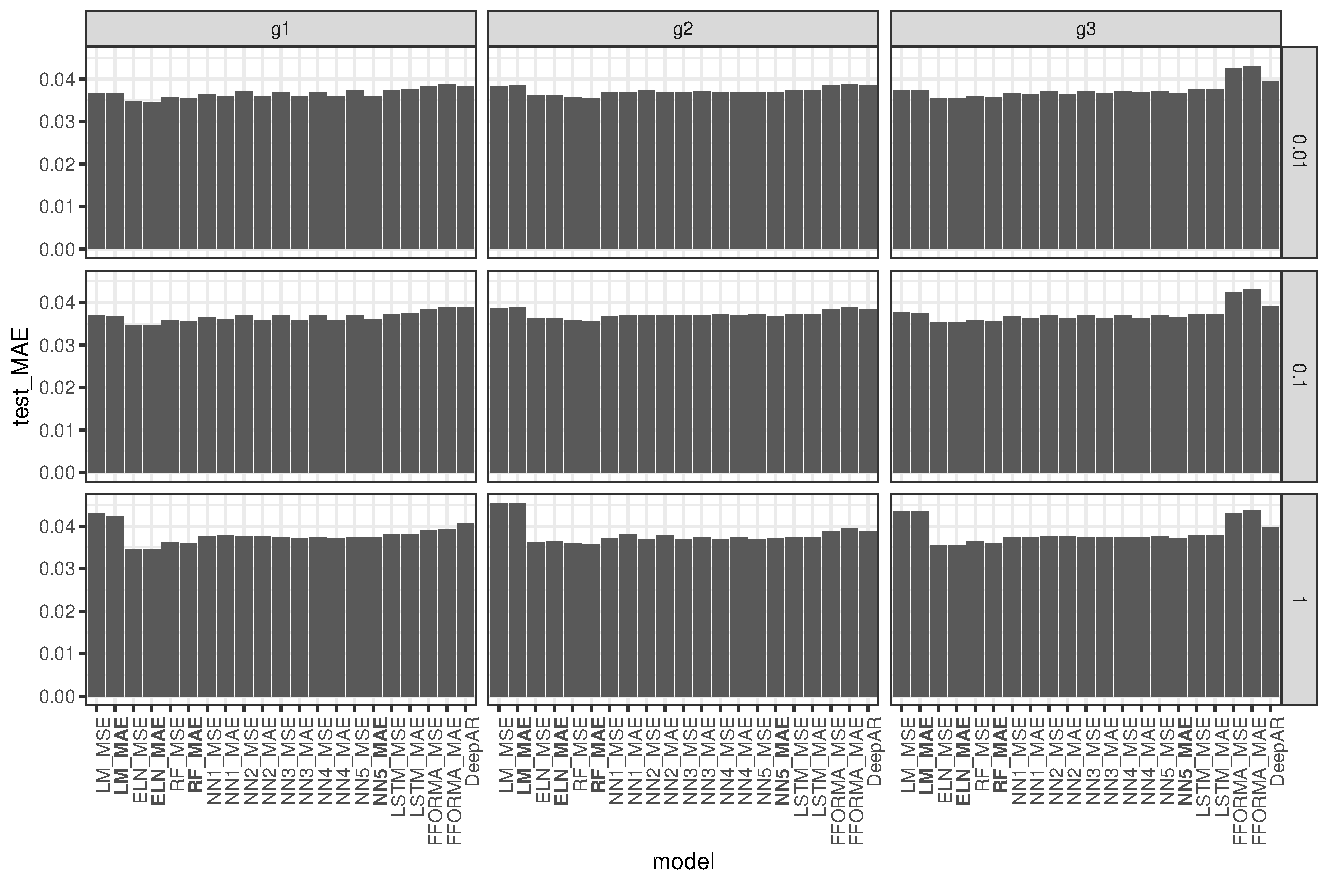
\includegraphics{simulation_test_mae.pdf}
		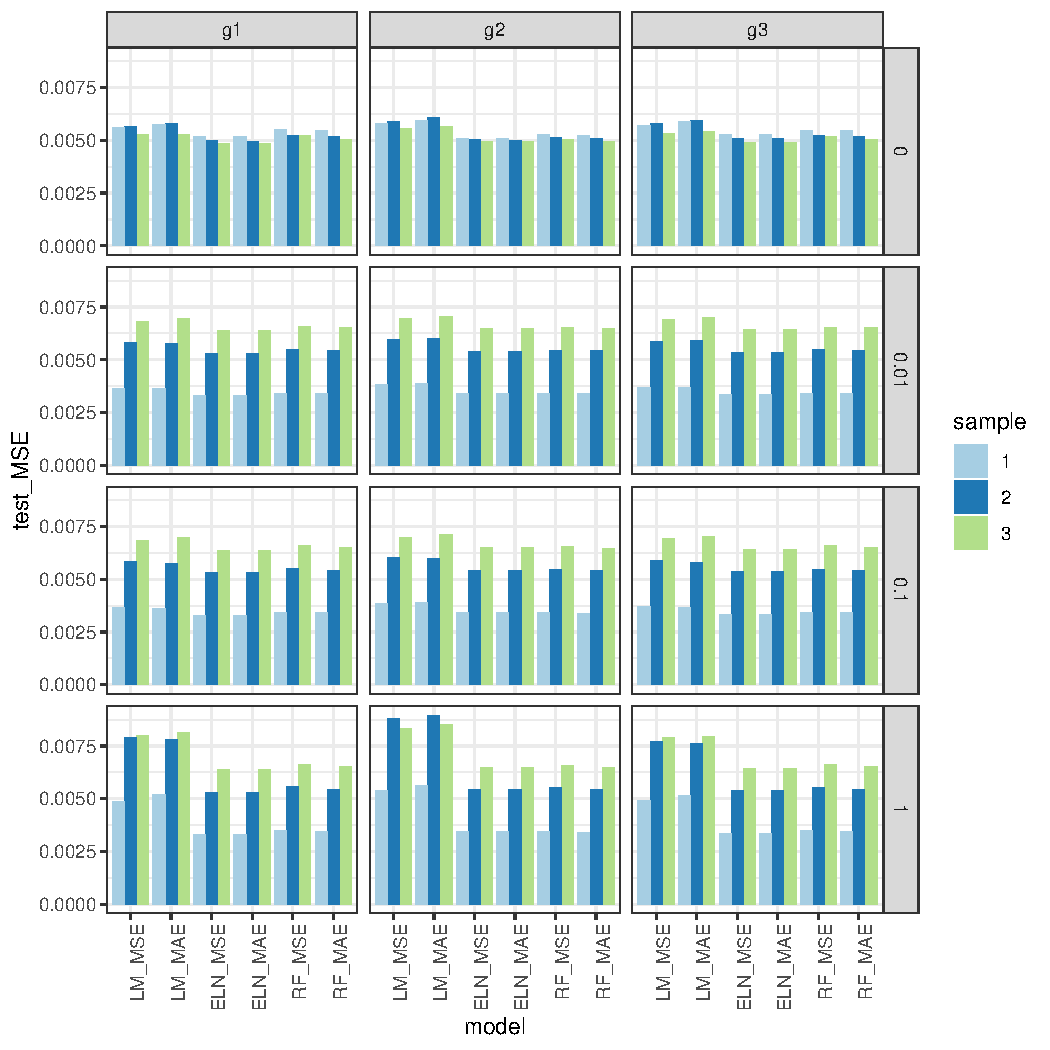
\includegraphics{simulation_test_mse.pdf}
	\end{center}
\end{table}

\begin{figure}
	\caption{Simulation Variable Importance Plots}
	\begin{center}
		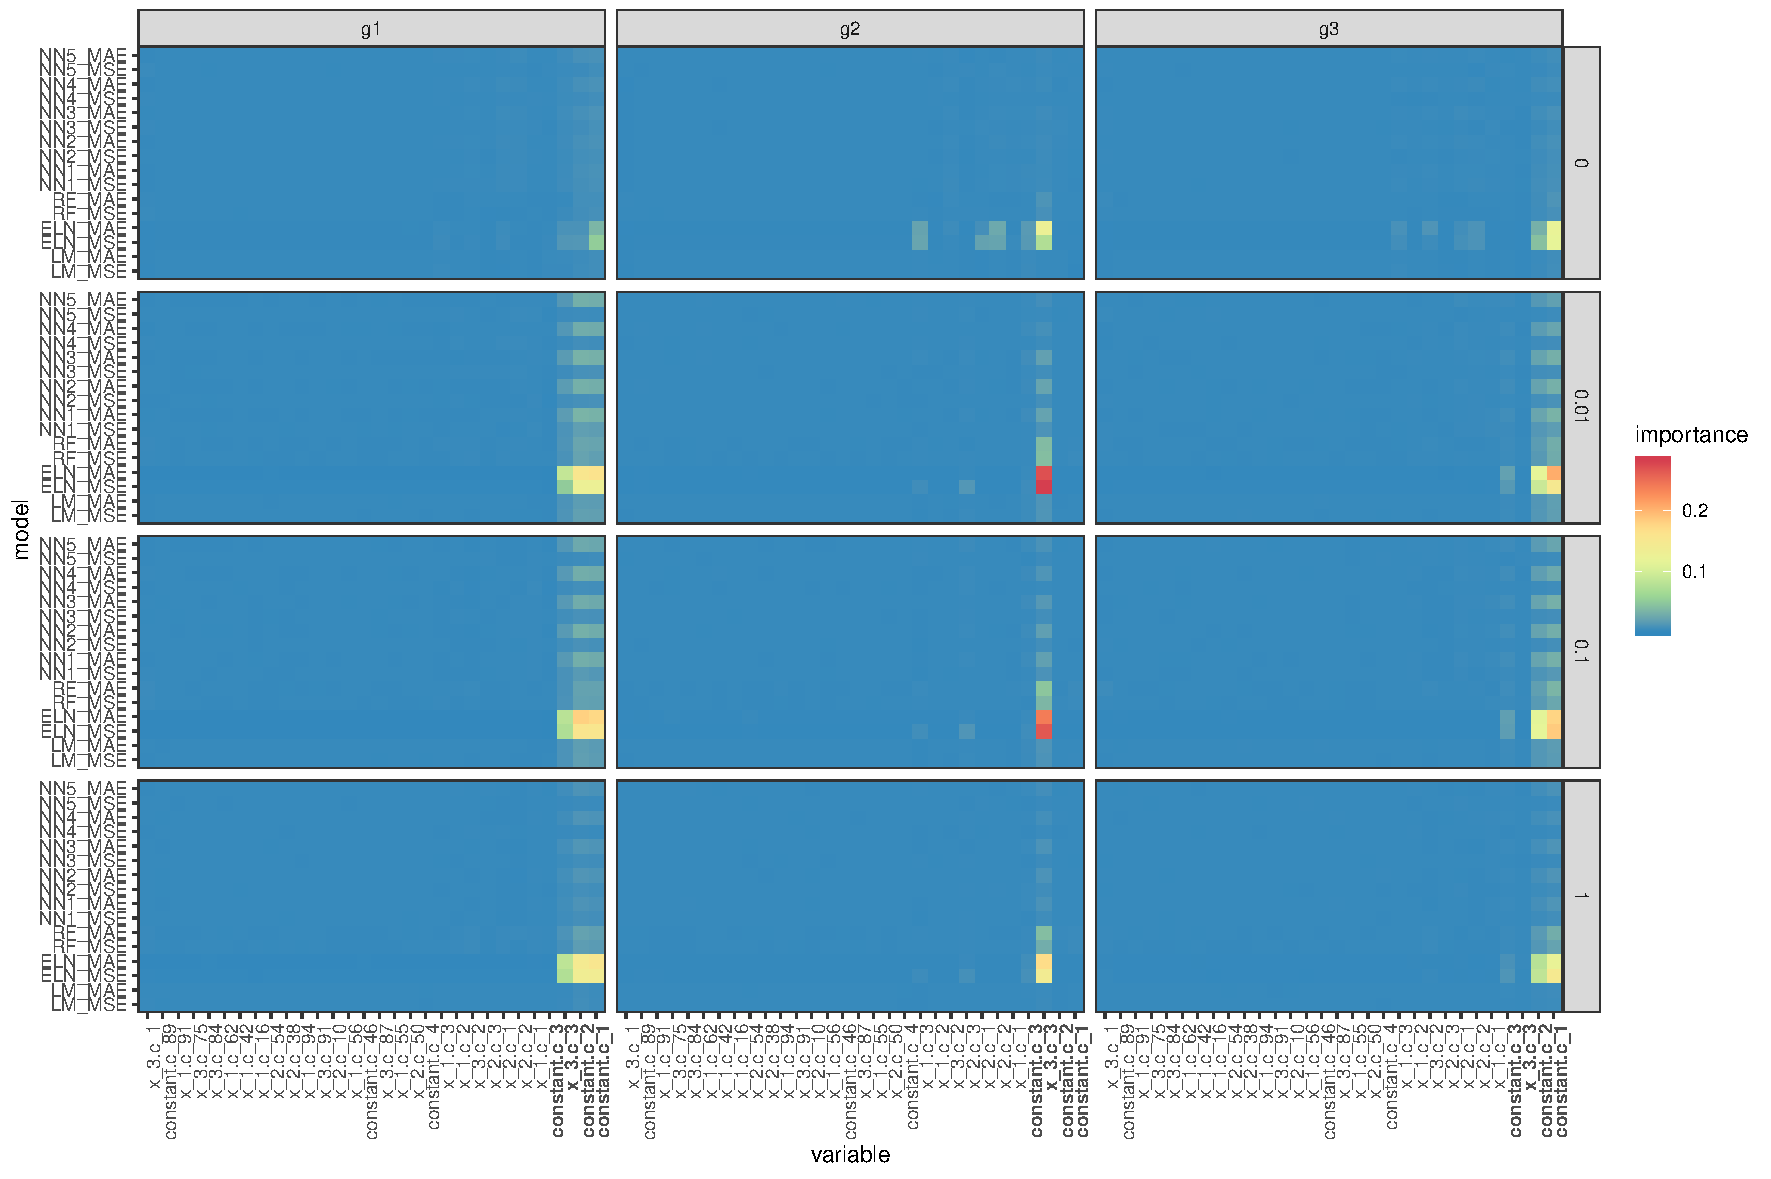
\includegraphics{simulation_ave_vi_plot.pdf}
		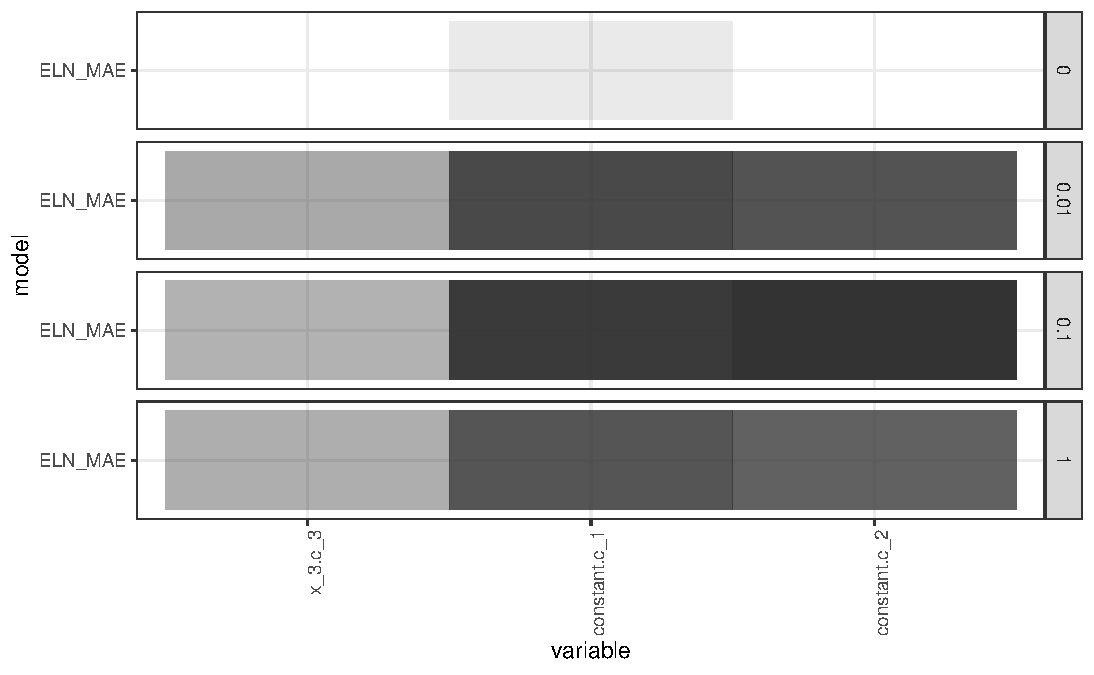
\includegraphics{simulation_g1_vi_plot.pdf}
		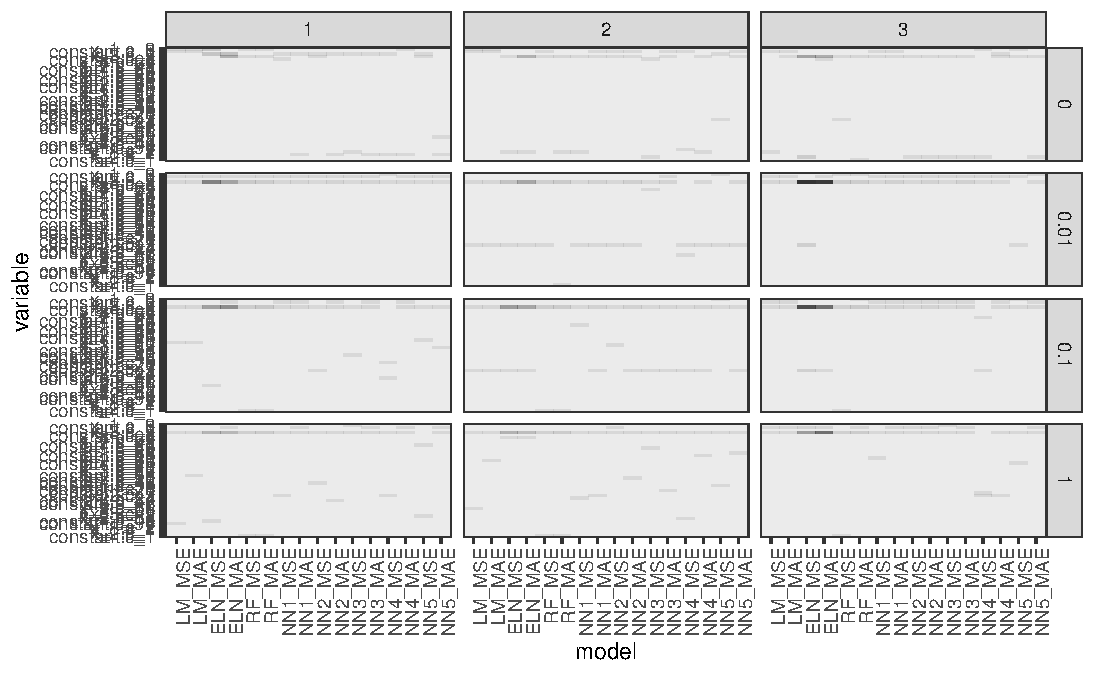
\includegraphics{simulation_g2_vi_plot.pdf}
		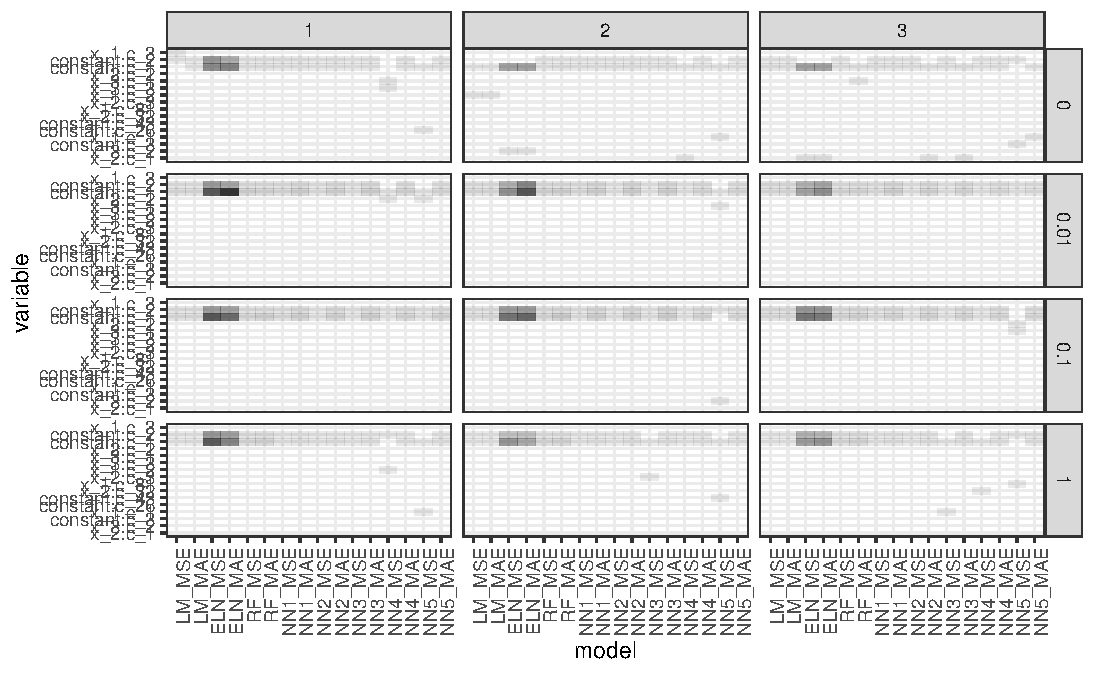
\includegraphics{simulation_g3_vi_plot.pdf}
	\end{center}
\end{figure}

\begin{table}
	\caption{Diebold Mariano Tests for Simulation Study}
\end{table}

%% Basic overview of results



\subsubsection{Linear Models}

The linear models performed very well in simple linear settings, with notably deteriorating performance as the specifications became more complex. They struggled greatly with cross sectional correlation even in specifications with no cross sectional correlation, as noted by the fact that they identify correlated interaction terms. When cross sectional correlation was increased

The introduction of non-linear interactions in the data generating process affected its performance, though it was still able to pick out transformations such as sgn and logit functions. This is likely due to these transformations not changing the direction of their terms.

\subsubsection{Penalized Linear Models}

The penalized linear models had markedly better performance than the linear models, though this was only apparent for more complex model specifications. 

Of particular note is the instability of the optimal hyperparameter as the validation set moved forward in time. It was quite common to see optimal $\alpha$ values that changed from 1 (equivalent to the sparse case of LASSO regression), to 0.01 (almost equivalent to dense case of ridge regression). Increasing the size of the validation set seemed to help a little, but not by a lot. 

Similarly to the linear models, penalized linear models which minimized mean absolute error (corresponding to quantile regression) offered consistent improvements over their mean squared error versions.

\subsubsection{Random Forests}

The random forests exhibited higher performance and robustness compared the linear and penalized linear models.

The random forests struggle greatly with determining variable importance in the presence of cross sectional correlation. This is to be expected, likely due to how the random forest algorithms work. Recall that the random forest algorithm is an ensemble of tree models, with each tree model only having access to a subset of all available predictors. If this subset does not include the true data generating predictor, that particular tree will likely select the predictors which have the highest correlation with the true data generating predictor instead. Thus, the resulting ensemble model is likely to believe that cross sectionally correlated predictors are important.

Very computationally intensive, so only a conservative grid of hyperparameters was able to be implemented. In particular, a low ntree parameter was used for feasibility, and it was not feasible to explore which value of ntree stopped improving performance. It is generally recommended to set the ntree parameter as high as computationally feasible, as doing so typically only increases performance. This means that there is possibly more room for higher performance from random forest models.

\subsubsection{Neural Networks}



\section{Empirical Data}

\subsection{Data}

% Description of original dataset
% mention how these variables are already adjusted for lags
We mimic the data procedure of \cite{gu_empirical_2018}. This means that we obtain the dataset provided by Gu on his website. This dataset sample begins in March 1957 (the start date of the S\&P 500) and ends in December 2016, totalling 60 years. It contains 94 stock level characteristics: 61 updated annually, 13 updated quarterly and 20 updated monthly, in addition to 74 industry dummies corresponding the the first two digits of the Standard Industrial Classification (SIC) codes. It is noted that this dataset contains all securities traded, including those with a CRSP share code other than 10 or 11 and thus includes instruments such as REITs and mutual funds, and those with a share price of less than \$5.

% Begin Cleaning

To reduce the size of the dataset and increase feasibility, the dataset was filtered so that only stocks traded primarily on NASDAQ were included (using the PRIMEXCH variable from WRDS). Then, penny stocks (also referred to as microcaps in the literature) with a stock price of less than \$5 were filtered out, as is commonly done in the literature to reduce variability. Stocks without a share code of 10 or 11 (referring to equities) were filtered out, so that securities that are not equities were not included (such as REITs and trust funds). The dataset is provided in a monthly format, which means that many of the factors which are updated only quarterly or annually have very low levels of variability, which can lead to misleading results in the model fitting process. The achieve of a balance between having a dataset with enough data points and variability among factors, the dataset was converted to a quarterly format. Quarterly returns were then constructed using the PRC variable according to actual returns (ie not logged differences):

\begin{equation}
	RET_t = \frac{PRC_t PRC_{t-1}}{PRC_{t-1}}
\end{equation}

%% Process in terms of pipes
% filter to only contain NASDAQ, share code = 10 or 11, PRC > $5, drop PRC = 0 (indicates not enough datain WRDS), drop industry dummies
% Convert to quarterly format so that dataset is smaller and more feasible
% Also helps with maintaing high variability in factors, as majority of these are updated annually
% Quarterly returns were then constructed using non-log process. May have slight differents compared to log version, and ignored dividend effect on prices. Should not have large differences
% Filter by time such that missing data is not so much of an issue. Noted that beginning from 1993 Q3 data quality improves dramatically, therefore filtered to start from 1993 Q3
% Drop any columns that had more than 20% missing
% Summarise data at this point
% Then, do cross sectional imputation of medians to fill in missing
% No normalization was done at this stage. Instead, each column was normalized for only the elasticnet and neural network methods

% Welch Goyal Data
% Quarterly version of Welch Goyal data was used
% New factor were constructed from this dataset, as with Gu et al
% Lagged by one period to be consistent with timing of other factors
% Treasury bill obtained to proxy for risk free rate of return to construct excess returns

We then follow \cite{gu_empirical_2018} and construct eight macroeconomic factors following the variable definitions in \cite{welch_comprehensive_2008}: dividend-price ratio (dp), earnings-price ratio (ep), book-to-market ratio (bm), net equity expansion (ntis), Treasury-bill rate (tbl), term spread (tms), default spread (dfy) and stock variance (svar). The treasury bill rate was also used from this source to construct excess quarterly returns. 

The two sets of factors were then combined according to \ref
 
As the individual and macroeconomic factors can have similar names, individual and macroeconomic factors were prefixed with ind\_ and macro\_ respectively.

% Splitting Scheme
% Similar splitting scheme to simulation study used
% Training:Validation size ratio of 1.5, growing and moving forwards by 1 year
% To maintain feasibility, only 3 samples were conducted


We detail our cleaning procedure of this dataset. To reduce the size and maintain computational feasibility, only shares traded on the NASDAQ exchange was included (filtered out using the PRIMEXCH variable). The majority of the characteristics included in the dataset are only updated annually, resulting in many rows having column values that remained constant for multiple time periods. To increase the variability yet also maintain a large enough number of time periods, quarterly returns were constructed. This also had the benefit of decreasing the dataset size for computational feasibility. 

The full details of these factors are available in table X.

There exists a significant amount of missing data in the dataset. The dataset's columns were first examined, and any characteristics that had over 20\% of their data were removed. However, as the amount of missing data increases dramatically going further back in time, a balance between using more periods at the cost of removing more characteristics versus using less periods but keeping more characteristics was needed. In the end, it was decided that any data before 1993 Q2 was to be filtered out, as there was a noticeable increase in data availability after this period.

Throughout all methods and analysis we define the baseline set of covariates as:

\begin{equation}
z_{i,t} = (1, x_t)' \otimes c_{i, t}
\end{equation}

where $c_{i,t}$ is a $P_c$ matrix of characteristics for each stock $i$, and $(1, x_t)'$ is a $P_x \times 1$ vector of macroeconomic predictors. $z_{i,t}$ is therefore a $P_x P_c$ vector of features for predicting individual stock returns and includes interactions between stock level characteristics and macroeconomic variables. The total number of covariates in this baseline set is $94 \times (8 + 1) + 74 = 920$.

The dataset was not normalized for all methods, as only penalized regression and neural networks are affected by normalization. For these two methods, the dataset was normalized such that each predictor column had 0 mean and 1 variance.

The final dataset spanned from 1993 Q3 to 2016 Q6 with ~20,000

\subsection{Empirical Data Model Fitting and Methodology Differences}

We detail our model fitting procedure used specifically for the empirical dataset.

We try to mimic the procedure used in the simulation study. This means that the dataset was split such that the training and validation sets were split such that the training set was 1.5 times the length of the validation set, in order to predict a test set that is one year in length.

\subsection{Empirical Data Results}

%% Empirical Results Data Table
% latex table generated in R 3.6.1 by xtable 1.8-4 package
% Thu Oct 24 17:04:52 2019
\begin{longtable}{rrlrrrrrrrrrrrr}
  \hline
 & Sample & model & train\_MAE & train\_MSE & train\_RMSE & train\_RSquare & validation\_MAE & validation\_MSE & validation\_RMSE & validation\_RSquare & test\_MAE & test\_MSE & test\_RMSE & test\_RSquare \\ 
  \hline
1 &   1 & LM\_MSE & 0.15 & 0.06 & 0.24 & 0.34 & 0.16 & 0.06 & 0.23 & -0.13 & 0.13 & 0.03 & 0.18 & 0.18 \\ 
  2 &   1 & LM\_MAE & 0.16 & 0.06 & 0.24 & 0.36 & 0.16 & 0.05 & 0.23 & -0.07 & 0.13 & 0.04 & 0.19 & 0.13 \\ 
  3 &   1 & ELN\_MSE & 0.16 & 0.06 & 0.25 & 0.32 & 0.12 & 0.03 & 0.18 & 0.34 & 0.11 & 0.03 & 0.17 & 0.27 \\ 
  4 &   1 & ELN\_MAE & 0.16 & 0.06 & 0.25 & 0.32 & 0.12 & 0.03 & 0.18 & 0.36 & 0.11 & 0.03 & 0.17 & 0.28 \\ 
  5 &   1 & RF\_MSE & 0.10 & 0.03 & 0.16 & 0.71 & 0.14 & 0.04 & 0.20 & 0.21 & 0.11 & 0.03 & 0.17 & 0.27 \\ 
  6 &   1 & RF\_MAE & 0.11 & 0.03 & 0.19 & 0.62 & 0.13 & 0.03 & 0.18 & 0.34 & 0.11 & 0.03 & 0.17 & 0.28 \\ 
  7 &   1 & NN1\_MSE & 0.16 & 0.06 & 0.25 & 0.32 & 0.14 & 0.04 & 0.20 & 0.16 & 0.13 & 0.04 & 0.19 & 0.10 \\ 
  8 &   1 & NN1\_MAE & 0.16 & 0.06 & 0.25 & 0.30 & 0.15 & 0.04 & 0.21 & 0.13 & 0.13 & 0.04 & 0.19 & 0.15 \\ 
  9 &   1 & NN2\_MSE & 0.16 & 0.06 & 0.25 & 0.31 & 0.14 & 0.04 & 0.20 & 0.15 & 0.14 & 0.04 & 0.20 & 0.01 \\ 
  10 &   1 & NN2\_MAE & 0.16 & 0.06 & 0.25 & 0.30 & 0.14 & 0.04 & 0.20 & 0.18 & 0.12 & 0.03 & 0.18 & 0.19 \\ 
  11 &   1 & NN3\_MSE & 0.17 & 0.06 & 0.25 & 0.30 & 0.15 & 0.04 & 0.20 & 0.14 & 0.15 & 0.04 & 0.21 & -0.05 \\ 
  12 &   1 & NN3\_MAE & 0.16 & 0.06 & 0.25 & 0.31 & 0.15 & 0.04 & 0.21 & 0.11 & 0.13 & 0.03 & 0.19 & 0.16 \\ 
  13 &   1 & NN4\_MSE & 0.16 & 0.06 & 0.25 & 0.31 & 0.14 & 0.04 & 0.21 & 0.14 & 0.13 & 0.04 & 0.19 & 0.11 \\ 
  14 &   1 & NN4\_MAE & 0.16 & 0.07 & 0.26 & 0.28 & 0.14 & 0.04 & 0.20 & 0.15 & 0.12 & 0.03 & 0.19 & 0.17 \\ 
  15 &   1 & NN5\_MSE & 0.17 & 0.07 & 0.26 & 0.26 & 0.15 & 0.04 & 0.21 & 0.13 & 0.14 & 0.04 & 0.20 & 0.02 \\ 
  16 &   1 & NN5\_MAE & 0.16 & 0.06 & 0.25 & 0.32 & 0.15 & 0.04 & 0.21 & 0.13 & 0.12 & 0.03 & 0.18 & 0.18 \\ 
  17 &   2 & LM\_MSE & 0.15 & 0.06 & 0.24 & 0.34 & 0.16 & 0.05 & 0.23 & -0.08 & 0.19 & 0.06 & 0.25 & -0.49 \\ 
  18 &   2 & LM\_MAE & 0.15 & 0.06 & 0.24 & 0.36 & 0.16 & 0.05 & 0.23 & -0.07 & 0.20 & 0.07 & 0.26 & -0.60 \\ 
  19 &   2 & ELN\_MSE & 0.16 & 0.06 & 0.24 & 0.32 & 0.12 & 0.03 & 0.18 & 0.34 & 0.11 & 0.03 & 0.17 & 0.34 \\ 
  20 &   2 & ELN\_MAE & 0.15 & 0.06 & 0.24 & 0.32 & 0.12 & 0.03 & 0.18 & 0.35 & 0.11 & 0.03 & 0.17 & 0.34 \\ 
  21 &   2 & RF\_MSE & 0.09 & 0.02 & 0.14 & 0.78 & 0.14 & 0.04 & 0.19 & 0.26 & 0.13 & 0.03 & 0.18 & 0.20 \\ 
  22 &   2 & RF\_MAE & 0.11 & 0.04 & 0.19 & 0.59 & 0.13 & 0.03 & 0.18 & 0.34 & 0.12 & 0.03 & 0.17 & 0.29 \\ 
  23 &   2 & NN1\_MSE & 0.16 & 0.06 & 0.25 & 0.32 & 0.15 & 0.04 & 0.20 & 0.15 & 0.15 & 0.04 & 0.21 & -0.01 \\ 
  24 &   2 & NN1\_MAE & 0.16 & 0.06 & 0.25 & 0.29 & 0.14 & 0.04 & 0.20 & 0.19 & 0.14 & 0.04 & 0.20 & 0.09 \\ 
  25 &   2 & NN2\_MSE & 0.16 & 0.06 & 0.25 & 0.31 & 0.15 & 0.04 & 0.21 & 0.12 & 0.14 & 0.04 & 0.19 & 0.13 \\ 
  26 &   2 & NN2\_MAE & 0.16 & 0.06 & 0.25 & 0.30 & 0.14 & 0.04 & 0.20 & 0.17 & 0.15 & 0.04 & 0.21 & 0.00 \\ 
  27 &   2 & NN3\_MSE & 0.16 & 0.06 & 0.25 & 0.31 & 0.15 & 0.04 & 0.21 & 0.13 & 0.17 & 0.06 & 0.24 & -0.30 \\ 
  28 &   2 & NN3\_MAE & 0.16 & 0.06 & 0.25 & 0.30 & 0.14 & 0.04 & 0.20 & 0.17 & 0.13 & 0.04 & 0.19 & 0.15 \\ 
  29 &   2 & NN4\_MSE & 0.16 & 0.06 & 0.25 & 0.32 & 0.14 & 0.04 & 0.20 & 0.17 & 0.15 & 0.04 & 0.21 & -0.05 \\ 
  30 &   2 & NN4\_MAE & 0.16 & 0.07 & 0.26 & 0.26 & 0.14 & 0.04 & 0.20 & 0.20 & 0.13 & 0.04 & 0.19 & 0.17 \\ 
  31 &   2 & NN5\_MSE & 0.16 & 0.07 & 0.26 & 0.26 & 0.15 & 0.04 & 0.21 & 0.14 & 0.12 & 0.03 & 0.18 & 0.21 \\ 
  32 &   2 & NN5\_MAE & 0.16 & 0.07 & 0.26 & 0.26 & 0.14 & 0.04 & 0.19 & 0.24 & 0.12 & 0.03 & 0.18 & 0.25 \\ 
  33 &   3 & LM\_MSE & 0.15 & 0.06 & 0.24 & 0.34 & 0.14 & 0.04 & 0.20 & 0.17 & 0.15 & 0.05 & 0.23 & -0.15 \\ 
  34 &   3 & LM\_MAE & 0.15 & 0.05 & 0.23 & 0.36 & 0.15 & 0.05 & 0.22 & 0.04 & 0.16 & 0.06 & 0.24 & -0.22 \\ 
  35 &   3 & ELN\_MSE & 0.15 & 0.06 & 0.24 & 0.33 & 0.13 & 0.03 & 0.18 & 0.33 & 0.11 & 0.03 & 0.17 & 0.37 \\ 
  36 &   3 & ELN\_MAE & 0.15 & 0.06 & 0.24 & 0.32 & 0.12 & 0.03 & 0.18 & 0.35 & 0.11 & 0.03 & 0.17 & 0.37 \\ 
  37 &   3 & RF\_MSE & 0.09 & 0.02 & 0.15 & 0.75 & 0.13 & 0.03 & 0.18 & 0.32 & 0.12 & 0.03 & 0.18 & 0.30 \\ 
  38 &   3 & RF\_MAE & 0.11 & 0.03 & 0.19 & 0.59 & 0.12 & 0.03 & 0.18 & 0.36 & 0.11 & 0.03 & 0.17 & 0.35 \\ 
  39 &   3 & NN1\_MSE & 0.16 & 0.06 & 0.24 & 0.31 & 0.15 & 0.04 & 0.21 & 0.14 & 0.15 & 0.05 & 0.22 & -0.09 \\ 
  40 &   3 & NN1\_MAE & 0.15 & 0.06 & 0.24 & 0.31 & 0.13 & 0.04 & 0.19 & 0.25 & 0.13 & 0.04 & 0.19 & 0.19 \\ 
  41 &   3 & NN2\_MSE & 0.16 & 0.06 & 0.24 & 0.31 & 0.15 & 0.04 & 0.20 & 0.17 & 0.14 & 0.04 & 0.20 & 0.10 \\ 
  42 &   3 & NN2\_MAE & 0.16 & 0.06 & 0.25 & 0.29 & 0.13 & 0.04 & 0.19 & 0.25 & 0.13 & 0.04 & 0.19 & 0.21 \\ 
  43 &   3 & NN3\_MSE & 0.16 & 0.06 & 0.25 & 0.29 & 0.15 & 0.05 & 0.21 & 0.09 & 0.16 & 0.05 & 0.23 & -0.16 \\ 
  44 &   3 & NN3\_MAE & 0.16 & 0.06 & 0.25 & 0.28 & 0.13 & 0.04 & 0.19 & 0.26 & 0.13 & 0.04 & 0.19 & 0.17 \\ 
  45 &   3 & NN4\_MSE & 0.16 & 0.06 & 0.24 & 0.30 & 0.14 & 0.04 & 0.20 & 0.18 & 0.13 & 0.04 & 0.20 & 0.10 \\ 
  46 &   3 & NN4\_MAE & 0.16 & 0.06 & 0.25 & 0.25 & 0.13 & 0.04 & 0.19 & 0.26 & 0.13 & 0.04 & 0.19 & 0.20 \\ 
  47 &   3 & NN5\_MSE & 0.16 & 0.06 & 0.24 & 0.31 & 0.14 & 0.04 & 0.20 & 0.17 & 0.15 & 0.05 & 0.22 & -0.05 \\ 
  48 &   3 & NN5\_MAE & 0.16 & 0.06 & 0.24 & 0.30 & 0.14 & 0.04 & 0.20 & 0.22 & 0.13 & 0.04 & 0.20 & 0.15 \\ 
   \hline
\hline
\caption{Empirical Data Results} 
\end{longtable}


\begin{figure}
	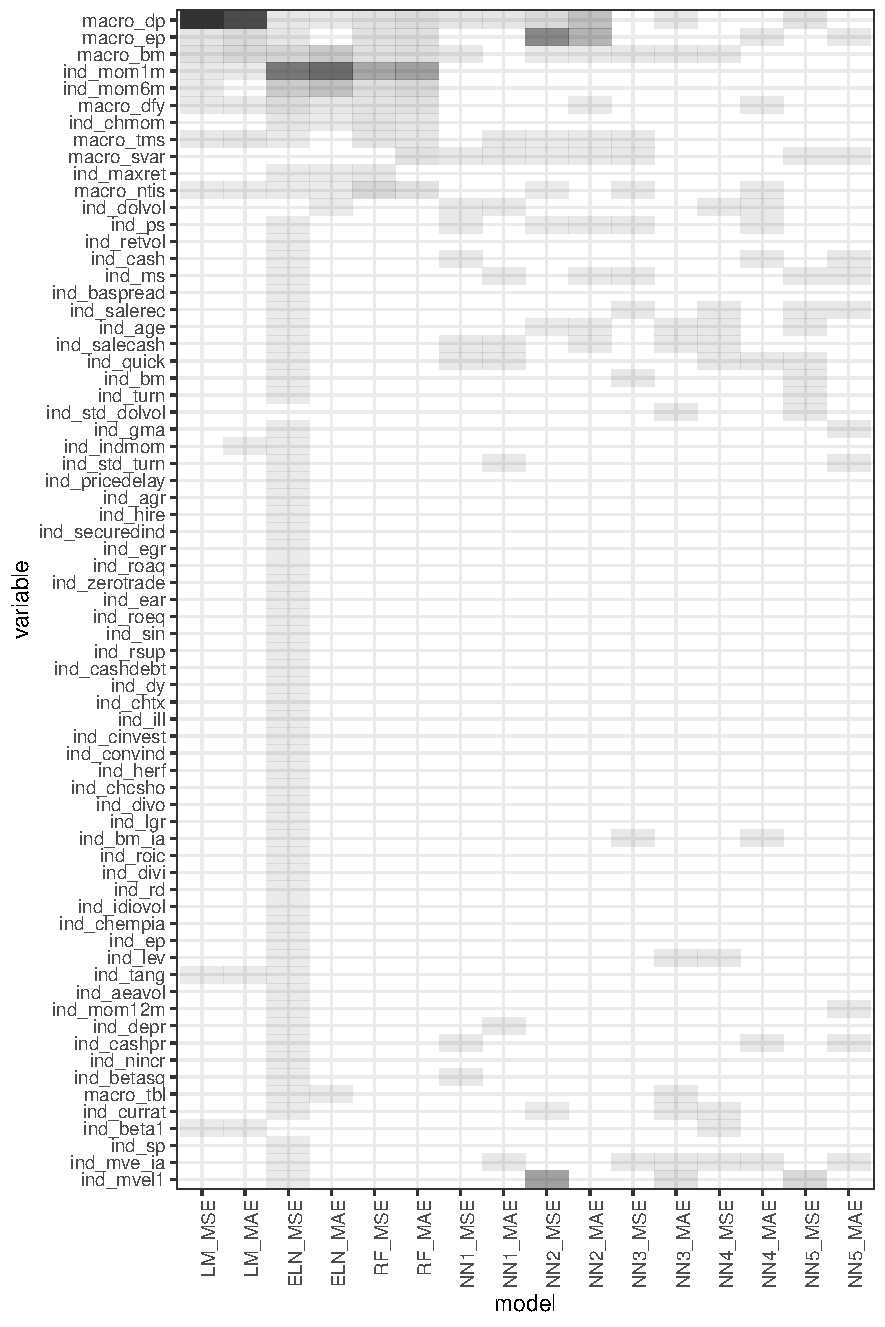
\includegraphics{empirical_sample_1_vi.pdf}
	\caption{Empirical Data Variable Importance Plots}
\end{figure}

\begin{figure}
	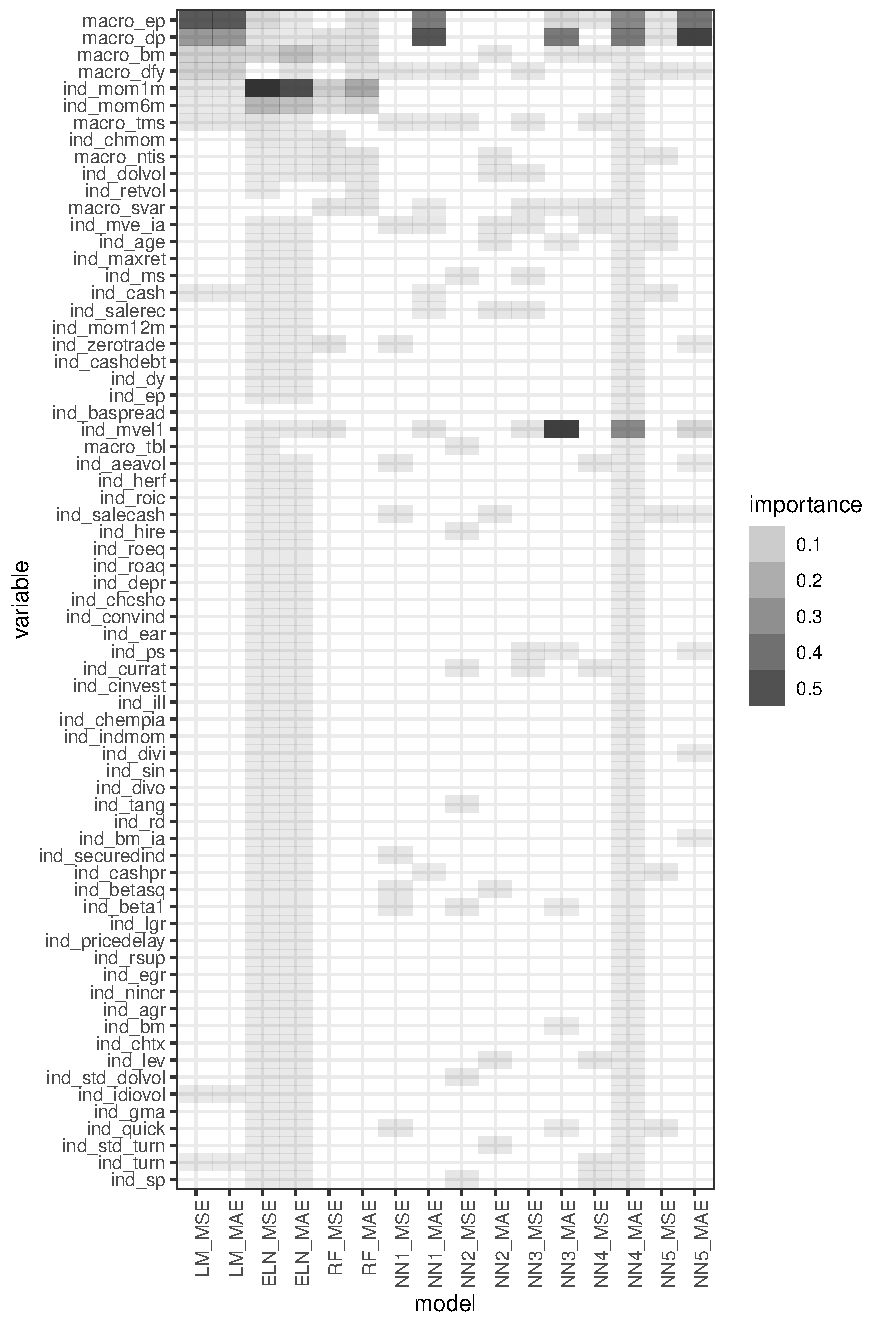
\includegraphics{empirical_sample_2_vi.pdf}
\end{figure}

\begin{figure}
	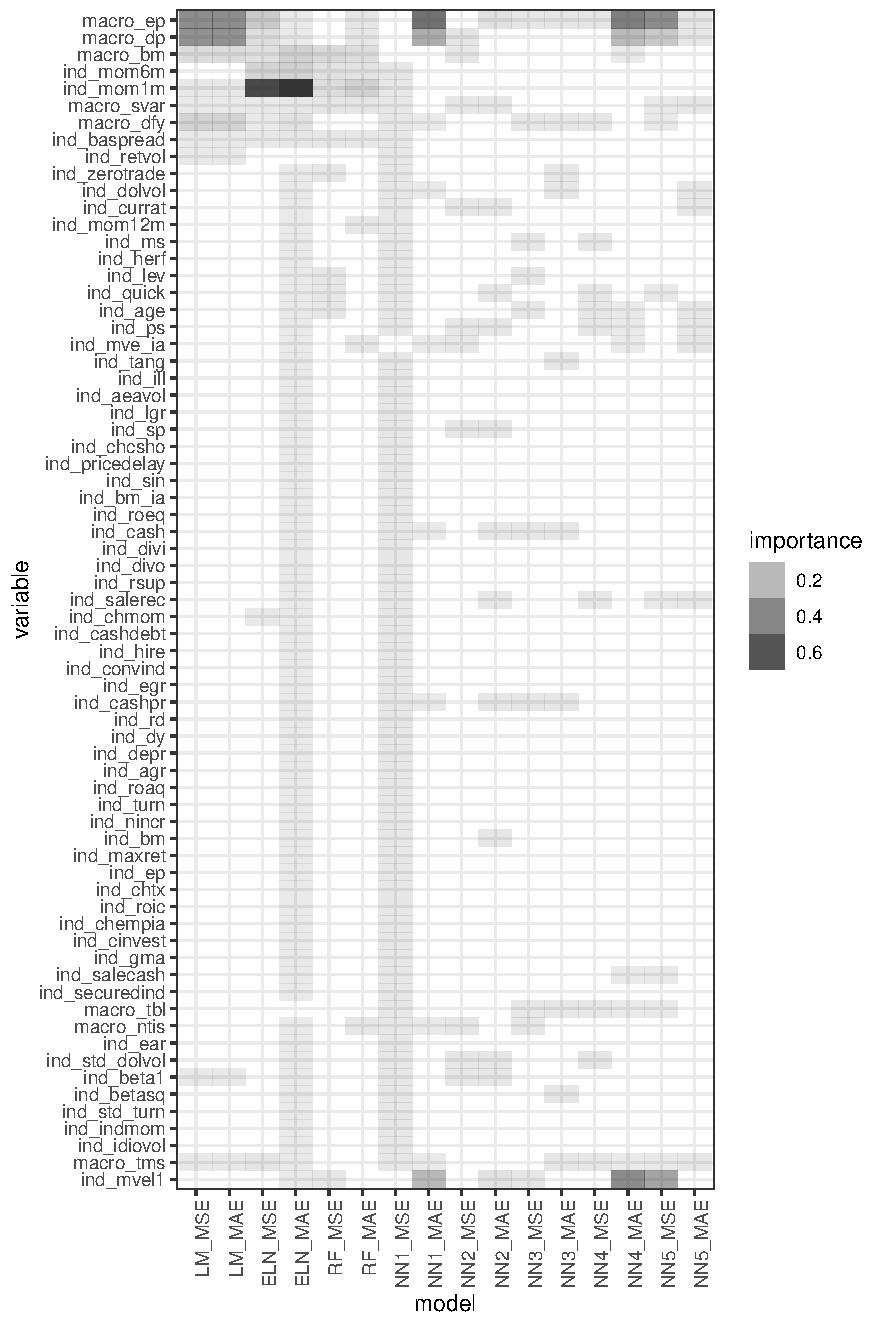
\includegraphics{empirical_sample_3_vi.pdf}
\end{figure}

\begin{figure}
	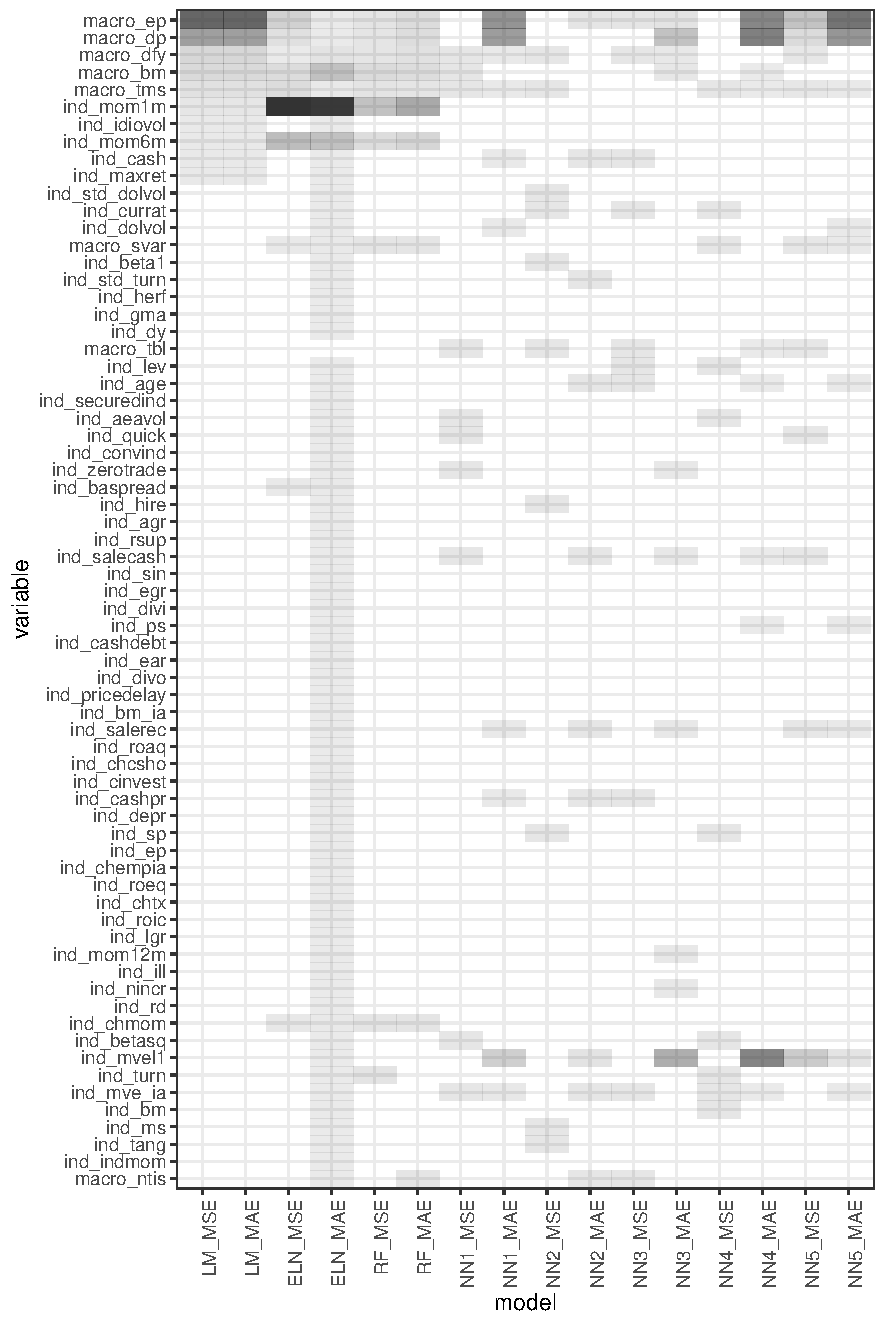
\includegraphics{empirical_sample_all_vi.pdf}
\end{figure}
	

\begin{table}
	\caption{Diebold Mariano Tests for Empirical Data}
\end{table}

In general, results from the simulation study were reproduced in the empirical study. We similarly see that the penalized linear models generally performing the best, with the random forest models offering slightly worse performance, occasionally outperforming penalized linear models. The neural networks offered lukewarm performance with the earlier training samples, but began to outperform random forests as the amount of training data increased.

Interestingly, 

\subsubsection{Linear Models}

The linear models typically had the worst performance among all the models.

\subsubsection{Penalized Linear Models}



\subsubsection{Random Forests}

Similar to the simulation study, the random forests overfitted the training sample by a large margin, offering the greatest performance by far for in sample forecasts.

\subsubsection{Neural Networks}

The neural networks offered lukewarm performance in the first two training samples, trailing behind the random forest and penalized linear models. 

\section{Limitations}

There were many limitations in this study.

Dataset limitations
The dataset 
As observed from both the simulation and empirical results, the neural networks' performance increases as the amount of training data does. 

Data splitting limitations
The data splitting scheme was decided in a pseudo-independent fashion: the training:validation length ratio of 1.5 was chosen to mimic the procedure of \cite{gu_empirical_2018}, in addition providing more stability for the neural network models. Crucially, this meant that no regards were given to large events affecting stock returns, including but not limited to the dot-com bubble, the 2008 Global Financial Crisis, and the 2015-2016 stock market sell-off. 

Model specification limitations
For each class of models considered, not all possible or reasonable specifications were explored. The linear and penalized linear models were not supplied with all possible higher order transformations, such as all possible pairwise interaction terms between all regressors as is the norm. This was mainly due to computational issues, as a model frame containing all possible pairwise interactions has exponentially higher memory requirements, in addition to computational feasibility. 

\section{Conclusion}



\section{Appendix}

\subsection{Data}

\begin{landscape}
	\footnotetext{The factor was included in the original dataset provided by \cite{gu_empirical_2018}, but was not used due to missing data issues}
	\begin{center}
		\begin{longtable}{llllllll} \hline 
			No. & Acronym & Firm Characteristic & Author(s) & Data Source & Frequency \\ \hline
			1 & absacc\footnotemark[\value{footnote}] & Absolute Accruals & 
				\cite{bandyopadhyay_accrual_2010} & Compustat & Annual \\
			2 & acc\footnotemark[\value{footnote}] & Working capital accruals & 
				\cite{sloan_stock_1996} & Compustat & Annual \\
			3 & aeavol & Abnormal earnings announcement volume & 
				\cite{lerman_high-volume_2008} & Compustat & Quarterly \\
			4 & age & \# years since first Compustat coverage & 
				\cite{jiang_information_2005} & Compustat & Annual \\
			5 & agr & Asset growth & 
				\cite{cooper_asset_2008} & Compustat & Annual \\
			6 & baspread & Bid-ask spread & 
				\cite{amihud_effects_1989} & Compustat & Monthly \\
			7 & beta & Beta & 
				\cite{fama_risk_1973} & Compustat & Monthly \\
			8 & betasq & Beta squared & 
				\cite{fama_risk_1973} & Compustat & Monthly \\
			9 & bm & Book-to-market & 
				\cite{rosenberg_persuasive_1985} & Compustat & Annual \\
			10 & bm\_ia & Industry-adjusted book to market & 
				\cite{asness_predicting_2000} & Compustat & Quarterly \\
			%%%%%%%%%%%%%%%%%%%%%%%%%%%%%%%%%%%%%%%%%%%%%%%%%%%%%%%%%%%%%%%%%%%%%%%%%%%%%%%
			11 & cash & Cash holdings & 
				\cite{palazzo_cash_2012} & Compustat & Annual \\
			12 & cashdebt & Cashflow to debt & 
				\cite{ou_financial_1989} & Compustat & Annual \\
			13 & cashpr & Cash productivity & 
				\cite{chandrashekar_productivity_2009} & Compustat & Annual \\
			14 & cfp\footnotemark[\value{footnote}] & Cashflow to price ratio & 
				\cite{desai_value-glamour_2004} & Compustat & Annual \\
			15 & cfp\_ia\footnotemark[\value{footnote}] & Industry-adjusted cashfow to price ratio & 
				\cite{asness_predicting_2000} & Compustat & Annual \\
			16 & chatoia\footnotemark[\value{footnote}] & Industry-adjusted change in asset turnover & 
				\cite{soliman_use_2008} & Compustat & Annual \\
			17 & chcsho & Change in shares outstanding & 
				\cite{pontiff_share_2008} & Compustat & Annual \\
			18 & chempia & Industry-adjusted change in employee & 
				\cite{asness_predicting_2000} & Compustat & Annual \\
			19 & chinv\footnotemark[\value{footnote}] & Change in inventory & 
				\cite{thomas_inventory_2002} & Compustat & Annual \\
			%%%%%%%%%%%%%%%%%%%%%%%%%%%%%%%%%%%%%%%%%%%%%%%%%%%%%%%%%%%%%%%%%%%%%%%%%%%%%%%
			20 & chmom & Change in 6-month momentum & 
				\cite{gettleman_acceleration_2006} & Compustat & Monthly \\
			21 & chpmia\footnotemark[\value{footnote}] & Industry-adjusted change in profit margin & 
				\cite{soliman_use_2008} & Compustat & Annual \\
			22 & chtx & Change in tax expense & 
				\cite{thomas_tax_2011} & Compustat & Quarterly \\
			23 & cinvest & Corporate investment & 
				\cite{titman_capital_2004} & Compustat & Quarterly \\
			24 & convind & Convertible debt indicator & 
				\cite{valta_strategic_2016} & Compustat & Annual \\
			25 & currat & Current ratio & 
				\cite{ou_financial_1989} & Compustat & Annual \\
			26 & depr & Depreciation / PP\&E & 
				\cite{holthausen_prediction_1992} & Compustat & Annual \\
			27 & divi & Dividend initiation & 
				\cite{michaely_price_1995} & Compustat & Annual \\
			28 & divo & Dividend omission & 
				\cite{michaely_price_1995} & Compustat & Annual \\
			29 & dolvol & Dollar trading volume & 
				\cite{chordia_trading_2001} & Compustat & Monthly \\
			%%%%%%%%%%%%%%%%%%%%%%%%%%%%%%%%%%%%%%%%%%%%%%%%%%%%%%%%%%%%%%%%%%%%%%%%%%%%%%%
			30 & dy & Dividend to price & 
				\cite{litzenberger_effects_1982} & Compustat & Annual \\
			31 & ear & Earnings announcement return & 
				\cite{brandt_earnings_2008} & Compustat & Quarterly \\
			32 & egr & Growth in common shareholder eq & 
				\cite{richardson_accrual_2005} & Compustat & Annual \\
			33 & ep & Earnings to price & 
				\cite{basu_investment_1977} & Compustat & Annual \\
			34 & gma & Gross profitability & 
				\cite{novy-marx_other_2013} & Compustat & Annual \\
			35 & grCAPX\footnotemark[\value{footnote}] & Growth in capital expenditures & 
				\cite{anderson_empirical_2006} & Compustat & Annual \\
			36 & grltnoa\footnotemark[\value{footnote}] & Growth in long term net operating assets & 
				\cite{fairfield_accrued_2003} & Compustat & Annual \\
			37 & herf & Industry sales concentration & 
				\cite{hou_industry_2006} & Compustat & Annual \\
			38 & hire & Employee growth rate & 
				\cite{belo_labor_2014} & Compustat & Annual \\
			39 & idiovol & Idiosyncratic return volatility & 
				\cite{ali_arbitrage_2003} & Compustat & Monthly \\
			%%%%%%%%%%%%%%%%%%%%%%%%%%%%%%%%%%%%%%%%%%%%%%%%%%%%%%%%%%%%%%%%%%%%%%%%%%%%%%%
			40 & ill & Illiquidity & 
				\cite{amihud_illiquidity_2002} & Compustat & Monthly \\
			41 & indmom & Industry momentum & 
				\cite{moskowitz_industries_1999} & Compustat & Monthly \\
			42 & invest\footnotemark[\value{footnote}] & Capital expenditures and inventory & 
				\cite{chen_better_2010} & Compustat & Annual \\
			43 & lev & Leverage & 
				\cite{bhandari_debt/equity_1988} & Compustat & Annual \\
			44 & lgr & Growth in long-term debt & 
				\cite{richardson_accrual_2005} & Compustat & Annual \\
			45 & maxret & Maximum daily return & 
				\cite{bali_maxing_2011} & Compustat & Monthly \\
			46 & mom12m & 12-month momentum & 
				\cite{jegadeesh_evidence_1990} & Compustat & Monthly \\
			47 & mom1 & 1-month momentum & 
				\cite{jegadeesh_returns_1993} & Compustat & Monthly \\
			48 & mom36m\footnotemark[\value{footnote}] & 36-month momentum & 
				\cite{jegadeesh_returns_1993} & Compustat & Monthly \\
			49 & mom6m & 6-month momentum & 
				\cite{jegadeesh_returns_1993} & Compustat & Monthly \\
			%%%%%%%%%%%%%%%%%%%%%%%%%%%%%%%%%%%%%%%%%%%%%%%%%%%%%%%%%%%%%%%%%%%%%%%%%%%%%%%
			50 & ms & Financial statement score & 
				\cite{mohanram_separating_2005} & Compustat & Quarterly \\
			51 & mvel1 & Size & 
				\cite{banz_relationship_1981} & Compustat & Monthly \\
			52 & mve\_ia & Industry-adjusted size & 
				\cite{asness_predicting_2000} & Compustat & Annual \\
			53 & nincr & Number of earnings increases & 
				\cite{barth_market_1999} & Compustat & Quarterly \\
			54 & operprof\footnotemark[\value{footnote}] & Operating profitability & 
				\cite{fama_five-factor_2015} & Compustat & Annual \\
			55 & orgcap\footnotemark[\value{footnote}] & Organizational capital & 
				\cite{eisfeldt_organization_2013} & Compustat & Annual \\
			56 & pchcapx\_ia\footnotemark[\value{footnote}] & Industry adjusted \% change in capital expenditures & 
				\cite{abarbanell_abnormal_1998} & Compustat & Annual \\
			57 & pchcurrat\footnotemark[\value{footnote}] & \% change in current ratio & 
				\cite{ou_financial_1989} & Compustat & Annual \\
			58 & pchdepr\footnotemark[\value{footnote}] & \% change in depreciation & 
				\cite{holthausen_prediction_1992} & Compustat & Annual \\
			59 & pchgm\_pchsale\footnotemark[\value{footnote}] & \% change in gross margin - \% change in sales & 
				\cite{abarbanell_abnormal_1998} & Compustat & Annual \\
			%%%%%%%%%%%%%%%%%%%%%%%%%%%%%%%%%%%%%%%%%%%%%%%%%%%%%%%%%%%%%%%%%%%%%%%%%%%%%%%
			60 & pchquick\footnotemark[\value{footnote}] & \% change in quick ratio & 
				\cite{ou_financial_1989} & Compustat & Annual \\
			61 & pchsale\_pchinvt\footnotemark[\value{footnote}] & \% change in sales - \% change in inventory & 
				\cite{abarbanell_abnormal_1998} & Compustat & Annual \\
			62 & pchsale\_pchrect\footnotemark[\value{footnote}] & \% change in sales - \% change in A/R & 
				\cite{abarbanell_abnormal_1998} & Compustat & Annual \\
			63 & pchsale\_pchxsga\footnotemark[\value{footnote}] & \% change in sales - \% change in SG & 
				\cite{abarbanell_abnormal_1998} & Compustat & Annual \\
			64 & pchsaleinv\footnotemark[\value{footnote}] & \% change sales-to-inventory & 
				\cite{ou_financial_1989} & Compustat & Annual \\
			65 & pctacc\footnotemark[\value{footnote}] & Percent accruals & 
				\cite{hafzalla_percent_2011} & Compustat & Annual \\
			66 & pricedelay & Price delay & 
				\cite{hou_market_2005} & Compustat & Monthly \\
			67 & ps & Financial statements score & 
				\cite{piotroski_value_2000} & Categorical & Compustat & Annual \\
			68 & quick & Quick ratio & 
				\cite{ou_financial_1989} & Compustat & Annual \\
			69 & rd & R\&D increase & 
				\cite{eberhart_examination_2004} & Compustat & Annual \\
			%%%%%%%%%%%%%%%%%%%%%%%%%%%%%%%%%%%%%%%%%%%%%%%%%%%%%%%%%%%%%%%%%%%%%%%%%%%%%%%
			70 & rd\_mve\footnotemark[\value{footnote}] & R\&D to market capitalization & 
				\cite{guo_explaining_2006} & Compustat & Annual \\
			71 & rd\_sale\footnotemark[\value{footnote}] & R\&D to sales & 
				\cite{guo_explaining_2006} & Compustat & Annual \\
			72 & realestate\footnotemark[\value{footnote}] & Real estate holdings & 
				\cite{tuzel_corporate_2010} & Compustat & Annual \\
			73 & retvol & Return volatility & 
				\cite{ang_cross-section_2006} & Compustat & Monthly \\
			74 & roaq & Return on assets & 
				\cite{balakrishnan_post_2010} & Compustat & Quarterly \\
			75 & roavol\footnotemark[\value{footnote}] & Earnings volatility & 
				\cite{francis_costs_2004} & Compustat & Quarterly \\
			76 & roeq & Return on equity & 
				\cite{hou_digesting_2015} & Compustat & Quarterly \\
			77 & roic & Return on invested capital & 
				\cite{brown_productivity_2007} & Compustat & Annual \\
			78 & rsup & Revenue surprise & 
				\cite{kama_market_2009} & Compustat & Quarterly \\
			79 & salecash & Sales to cash & 
				\cite{ou_financial_1989} & Compustat & Annual \\
			%%%%%%%%%%%%%%%%%%%%%%%%%%%%%%%%%%%%%%%%%%%%%%%%%%%%%%%%%%%%%%%%%%%%%%%%%%%%%%%
			80 & saleinv\footnotemark[\value{footnote}] & Sales to inventory & 
				\cite{ou_financial_1989} & Compustat & Annual \\
			81 & salerec & Sales to receivables & 
				\cite{ou_financial_1989} & Compustat & Annual \\
			82 & secured\footnotemark[\value{footnote}] & Secured debt & 
				\cite{valta_strategic_2016} & Compustat & Annual \\
			83 & securedind & Secured debt indicator & 
				\cite{valta_strategic_2016} & Compustat & Annual \\
			84 & sgr\footnotemark[\value{footnote}] & Sales growth & 
				\cite{barbee_jr_salesprice_1996} & Compustat & Annual \\
			85 & sin & Sin stocks & 
				\cite{hong_price_2009} & Compustat & Annual \\
			86 & sp & Sales to price & 
				\cite{barbee_jr_salesprice_1996} & Compustat & Annual \\
			87 & std\_dolvol & Volatility of liquidity (dollar trading volume) & 
				\cite{chordia_trading_2001} & Compustat & Annual \\
			88 & std\_turn & Volatility of liquidity (share turnover) & 
				\cite{chordia_trading_2001} & Compustat & Monthly \\
			89 & stdacc\footnotemark[\value{footnote}] & Accrual volatility & 
				\cite{bandyopadhyay_accrual_2010} & Compustat & Monthly \\
			%%%%%%%%%%%%%%%%%%%%%%%%%%%%%%%%%%%%%%%%%%%%%%%%%%%%%%%%%%%%%%%%%%%%%%%%%%%%%%%
			90 & stdcf\footnotemark[\value{footnote}] & Cashflow volatility & 
				\cite{huang_cross_2009} & Compustat & Quarterly \\
			91 & tang & Debt capacity/rm tangibility & 
				\cite{almeida_financial_2007} & Compustat & Quarterly \\
			92 & tb\footnotemark[\value{footnote}] & Tax income to book income & 
				\cite{lev_market-based_1982} & Compustat & Annual \\
			93 & turn & Share turnover & 
				\cite{datar_liquidity_1998} & Compustat & Monthly \\
			94 & zerotrade & Zero trading days & 
				\cite{liu_liquidity-augmented_2006} & Compustat & Monthly \\	
		\end{longtable}
	\end{center}
\end{landscape}

\newpage

\begin{table}
	\caption{Macroeconomic Factors}
	\begin{center}
	\begin{tabular}{lccc} \hline \hline
		No. & Acronym & Macroeconomic Factor \\ \hline \hline
		1 & macro\_dp & Dividend Price Ratio \\
		2 & macro\_ep & Earnings Price Ratio \\
		3 & macro\_bm & Book to Market Ratio \\
		4 & macro\_ntis & Net Equity Expansion \\
		5 & macro\_tbl & Treasury Bill Rate \\
		6 & macro\_tms & Term Spread \\
		7 & macro\_dfy & Default Spread \\
		8 & macro\_svar & Stock Variance \\
	\end{tabular}
	\end{center}
\end{table}

\subsection{Computational Details}
\label{Algorithms}

\subsubsection{Linear Models}

OLS used for fitting wrt MSE.

quantreg package used for fitting wrt MAE. (minimizing 0.5 quantile loss is equivalent to minimizing mae).

\subsubsection{Penalized Linear}

The package  was used to fit penalized regression models with respect to MSE and MAE.

This package efficiently calculates a regularization path of penalization values given a value for $\alpha$. This means that it is much more efficient to instead only supply a grid for $\alpha$, let the algorithm decide its own path of penalization values. The combination of these two parameters which produces the best results on the validation set were then chosen.

The more traditional method of supplying a grid of $\alpha$ and $\lambda$ was also implemented at first, and this was observed to give almost identical results to the above implementation, but at a much higher computational cost.

\subsubsection{Classification and Regression Trees}

For full details of the Classification and Regression Tree algorithm see \cite{breiman_classification_1984}. 

\begin{algorithm}[H]
	\SetAlgoLined
	Initialize \;
	\For{$d$ from 1 to $L$}{
		\For{$i$ in ${C_l(d-1), l = 1, \dots, 2^{d-1}}$}{
			For each feature $j = 1, 2, \dots, P,$ and each threshold level $\alpha$, define a split as $s = (j, \alpha)$ which divides $C_l(d-1)$ into $C_{left}$ and $C_{right}$:
			\begin{equation*}
				C_{left}s = \{z_j \leq \alpha\} \cap C_l(d-1); C_{right}s = \{z_j > \alpha\} \cap C_l(d-1)
			\end{equation*}
			
			Define the impurity function:
			\begin{equation*}
				\mathcal{L}(C, C_{left}, C_{right}) = \frac{|C_{left}|}{|C|}H(C_{left}) + \frac{|C_{right}|}{|C|}H(C_{right})
			\end{equation*}
			where
			\begin{equation*}
			H(C) = \frac{1}{|C|} \sum_{ }^{z_{i,t}\in C}(r_{i,t+1}-\theta)^2, \theta = \frac{1}{|C|} \sum_{z_{i,t}\in C}^{ }r_{i,t+1}
			\end{equation*}
			and $|C|$ denotes the number of observations in set C
			
			Find the optimal split
			\begin{equation*}
				s^* \leftarrow \underset{s}{argmin}\mathcal{L}(C(s),C_{left}(s),C_{right}(s))
			\end{equation*}
			Update nodes (partition the data):
			\begin{equation*}
				C_{2l-1}(d) \leftarrow C_{left}(s^*), C_{2l}(d) \leftarrow C_{right}(s^*)
			\end{equation*}
		}
	}
	\KwResult{The prediction of a regression tree is:
	\begin{equation*}
		g(z_{i,t};\theta,L) = \sum_{k=1}^{2^L}\theta_k\textbf{1}_{z_{i,t}\in C_k(L)}; \theta_k = \frac{1}{|C_{k}(L)|} \sum_{z_{i,t}\in C_k(L)}^{ }r_{i,t+1}
	\end{equation*}
	}
	\caption{Classification and Regression Tree}
\end{algorithm}

\subsubsection{Random Forest}

For full details of the Random Forest algorithm see \cite{breiman_random_2001}. 

\begin{algorithm}[H]
	\SetAlgoLined
	\For{$b$ from $1$ to $B$}{
		Draw bootstrap samples {$(z_{i,t},r_{i,t+1}),(i,t) \in Bootstrap(b)$} from the dataset\
		Grow a tree $T_b$ using Algorithm, using only a random subsample, say $\sqrt{P}$ of all features \
		Denote the resulting $bth$ tree as
		\begin{equation*}
			\hat{g}_b (z_{i,t},\hat{\theta}_b, L) = \sum_{k=1}^{2^L}\theta_b^k\textbf{1}_{z_{i,t}\in C_k(L)}
		\end{equation*}
	}
	\KwResult{The final random forest prediction is given by the output of all trees:
		\begin{equation*}
			\hat{g}_b (z_{i,t}; L, B) = \frac{1}{B} \sum_{b=1}^B \hat{g}_b (z_{i,t},\hat{\theta}_b, L)
		\end{equation*}
	}
	\caption{Random Forest}
\end{algorithm}

\subsubsection{Neural Networks}

Fit using {keras} package (cite)

ADAM algorithm for stochastic gradient descent and learning rate shrinkage as detailed by \cite{kingma_adam:_2014}.

\begin{algorithm}
	\SetAlgoLined
	Initialize $j = 0$, $\epsilon = \infty$ and select the patience parameter $p$ (max iterations)\
	
	\While{j < p}{
		Update $\theta$ using the training algorithm\
		Calculate the prediction error from the validation sample, denoted as \(\epsilon'\)\
		
		\eIf{\(\epsilon' < \epsilon\)}
			{\(j \leftarrow 0\)\
				
			 \(\epsilon \leftarrow \epsilon'\)\
			 
		     \(\theta' \leftarrow \theta\)}
	     	{\(j \leftarrow j+1\)}
	}
	\KwResult{$\theta'$ is the final parameter estimate}
	\caption{Early stopping via validation}
\end{algorithm}

Batch Normalization Algorithm as detailed by \cite{ioffe_batch_2015}.

\begin{algorithm}
	Input: Values of \(x\) for each activation over a batch \(\mathcal{B} = {x_1, x_2, \dots, x_N}\)
	
	\(\mu_\mathcal{B} \leftarrow \frac{1}{N} \sum_{i = 1}^{N}x_i\)
	
	\(\sigma_\mathcal{B}^2 \leftarrow \frac{1}{N} \sum_{i = 1}^{N}(x_i - \mu_\mathcal{B})^2\)
	
	\(\hat{x_i} \leftarrow \frac{x_i - \mu_\mathcal{B}}{\sqrt{\sigma_\mathcal{B}^2 + \epsilon}}\)
	
	\(y_i \leftarrow \gamma\hat{x_i} + \beta := BN_{\gamma, \beta}(x_i)\)
	
	\KwResult{\(y_i = BN_{\gamma, \beta}(x_i) : i = 1, 2, ..., N\)}
	\caption{Batch Normalization for one activation over one batch}
\end{algorithm}

\subsubsection{Tuning of Simulated Datasets}

The simulated datasets were tuned according to the following statistics: average individual time series R squared, average annualized volatility, and cross sectional R squared, and true/predictive R squared.

The methodology for evaluating average time series R squared and cross sectional R squared is consistent with that detailed by \cite{cochrane_asset_2005}. The steps are reproduced here for reference; for complete details refer to \cite{cochrane_asset_2005}.

First evaluate the following OLS model:

\begin{equation}
	R_{it} = a_i + \beta_i' f_{it} + \epsilon_{it} 
\end{equation}

where $f_{it}$ represents the \textit{true} factors in the returns process. The corresponding R-squared value for this time series regression is calculated across all stocks and averaged to yield the average time series R-Squared. 

A cross sectional regression for the risk premia is then run across assets of average returns on the factor coefficients:

\begin{equation}
	\bar{R_{it}} = \alpha_i = \beta_i' \lambda
\end{equation}

where the $\beta_i'$ are the estimated coefficients from each time series regressions run previously. The corresponding R squared for this regression is the cross sectional R squared.

The true R squared is a measure of signal to noise ratio i.e. how much of the returns data is due to 
This is simply calculated by running a pooled ordinary least squares regression on the entire panel, using the underlying g() as the "predictions.' The resulting R squared value is therefore a measure of how much of the panel can be explained by the g() term exclusive of any noise or error terms.

%%%%%%%%%%%%%%%%%%%%%%%%%%%%%%%%%%
%%BIBLIOGRAPHY
%%%%%%%%%%%%%%%%%%%%%%%%%%%%%%%%%%

\bibliographystyle{jfe}
\bibliography{Bibliography}

\end{document}